\documentclass[a4paper,11pt]{book}


\usepackage[top=2cm,bottom=2cm,left=2cm,right=2cm]{geometry}
\usepackage[pdftex]{graphicx} 
\usepackage{amssymb,amsmath,amsthm,amsfonts}
\usepackage{xspace}
\usepackage{tabularx}
\usepackage{indentfirst}
\usepackage{subfigure}
\usepackage[small]{caption}
\usepackage{eucal}
\usepackage{eso-pic}
\usepackage{url}
\usepackage{booktabs}
\usepackage{afterpage}
\usepackage{parskip}
\usepackage{listings}
\usepackage{fancyhdr}
\usepackage{textcomp}
\usepackage{cite}
\usepackage{multirow}
\usepackage[utf8]{inputenc}   
\usepackage[english]{babel}    
\usepackage{setspace}
\usepackage{graphicx,wrapfig,lipsum}
\usepackage{bm}
\pagestyle{fancy}




\begin{document}

\begin{titlepage}
\vspace{5mm}
\begin{figure}[hbtp]
\centering

\includegraphics[scale=.13]{logo_unipd.png}
\end{figure}
\vspace{5mm}
\begin{center}
{{\huge{\textsc{\bf UNIVERSIT\`A DEGLI STUDI DI PADOVA}}}\\}
\vspace{5mm}
{\Large{\bf Dipartimento di Fisica e Astronomia ``Galileo Galilei''}} \\
\vspace{5mm}
{\Large{\textsc{\bf Corso di Laurea in Fisica}}}\\
\vspace{20mm}
{\Large{\textsc{\bf Tesi di Laurea}}}\\
\vspace{30mm}
\begin{spacing}{3}
{\LARGE \textbf{Track reconstruction of trigger-less drift tubes chambers}}\\
\end{spacing}
\vspace{8mm}
\end{center}

\vspace{20mm}
\begin{spacing}{2}
\begin{tabular}{ l  c  c c c  cc c c c c  l }
{\Large{\bf Relatore}} &&&&&&&&&&& {\Large{\bf Laureando}}\\
{\Large{\bf Prof. Marco Zanetti}} &&&&&&&&&&& {\Large{\bf Mattia Pujatti}}\\
\end{tabular}
\end{spacing}
\vspace{15 mm}

\begin{center}
{\Large{\bf Anno Accademico 2018/2019}}
\end{center}
\end{titlepage}


\clearpage{\pagestyle{empty}\cleardoublepage}

\tableofcontents


\chapter*{Abstract}

A re-scaled and revisited version of the CMS drift tubes muon chambers has been designed to be used at beam tests and for
tomography applications. A set of chambers of this type have been produced at the INFN Legnaro Laboratory in 2018 and 2019. An
important feature of those detectors is their handiness, i.e. they can be arranged to best fit the experimental needs. It is therefore
important to develop a reconstruction algorithm flexible enough to address multiple geometrical configurations; at the same time,
dedicated suites have to be deployed to allow a fast determination of alignment and calibration constants. Furthermore, the readout
of those detectors do not require a trigger signal, i.e. (zero-suppressed) data are continuously sampled from the front-ends. In view
of an online analysis running on the unfiltered data, the track reconstruction must be fast, little sensitive to noise and developed with
software tools that can best fit in an online environment. The thesis work will focus on the development of algorithms which satisfy
the requirements listed above.




\part{The Physics behind the muon detectors}


\chapter{Track Detectors}
\section{Gaseous Ionization Detectors}
Drift chambers are part of the so-called gaseous ionization detectors, that exploit the passage of ionization radiation trough a gas to produce, for every interaction, electron-ion pairs. At the ends of these devices there are two electrodes, among which an appropriate potential difference is established, which allows to create a uniform and constant electric field inside the chamber. Ionization charges produced are drawn towards the ends of the machine (electrons to the anode and positive ions to the cathode) and collected by a circuit that generates a signal which will then be analyzed.\\
The different mobility of electrons respect to the ions one, makes the first ones arrive at their destination very early, and therefore it is often convenient to limit oneself to collecting only that type of charges, which in any case generate a sufficient signal that, in the worst case, can be amplified before the analysis.\\
The most used gases within these detectors are Boron, Helium and Argon, but in any case always substances in the gaseous state, because, although liquids and solids increase the number of possible interactions thanks to their greater density, at the same time they can limit the mobility of the ionization charge inside the chamber, causing collection delays and noisier signals. The advantage brought by these noble gases is due to the completeness of their electronic shells, which causes the energy of the particles to be dissipated almost entirely for ionization. Moreover, the lack of electronegativity prevents the capture of electrons and the harmful creation of negative ions.\\
Below, in figure \ref{fig:gas_ion_ch_scheme}, the operating scheme of an ionization detector is shown:\\

\begin{figure}[hbtp]
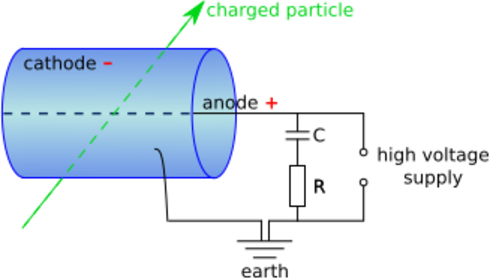
\includegraphics{pictures/gas_ion_det.pdf}
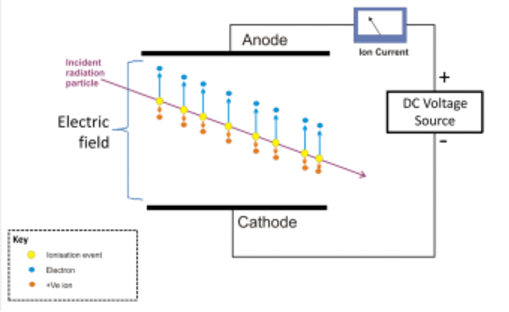
\includegraphics{pictures/gas_ion_det_2.pdf}
\caption{Scheme for a gaseous ionization chamber}
\label{fig:gas_ion_ch_scheme}
\end{figure}

Ionization electrons reach then the anode and, accumulating on the plates of the capacitance $C$, increase the tension on the resistance and they give rise to an impulsive signal trough it, which is electronically registered.\\

As is known, the potential variation on the condenser, and therefore indirectly that on resistance, is directly proportional to the charge variation accumulated on the plates ($\Delta Q = \Delta V/C$), which is just equal to the number of electrons collected in the anode. But the amount of charges collected in the anode will depend on the actual number of interactions occurred between the molecules of the gas present in the chamber and the ionizing particle, number to which, however, an appropriate amplification factor must be multiplied (that can be called $A$) which takes into account a possible secondary ionization. If the products of the first ionization aren't sufficiently energetic, it cannot be ruled out that the phenomenon may recur.\\
Named $n\cdot e$ the charges produced by first ionization, the height of the signal collected by the electronics is:
\[ \text{Pulse height = } \Delta V = A\frac{n\cdot e}{C} \]
It can be observed, for this type of detector, that the ionization charge depends heavily on the intensity of the electric field established within the apparatus, so much to define different regions of work, represented by the graph \ref{fig:ion_ch_work_regions}.\\

\begin{figure}[hbtp]
\centering
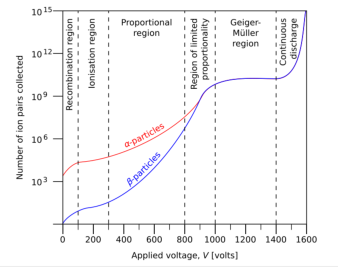
\includegraphics[scale=1.5]{pictures/work_region_det.pdf}
\caption{Ionization charge vs electric field intensity in a gaseous ionization chamber}
\label{fig:ion_ch_work_regions}
\end{figure}

The most important of these, the one which most radiation detectors operate on, it's the \textit{proportional region}, characterized by a strong potential gradient next to the anode, which allows the formation of a phenomenon known as \textit{Townsend avalanche}. The presence of a sufficiently intense electric field allows the ionization electrons to accelerate and, hitting each other or with the gas molecules, to acquire enough energy to produce another ionization and a consequent one avalanche of new charges.\\
The advantage of having an avalanche is that the charge is multiplied for a very large factor (typically around $10^4$ / $10^6$) and therefore the signal that is induced on the anode is very intense, especially \textit{proportional} to the charge released during the first ionization.\\



\subsection{Proportional Counters}
Detectors that work in proportional region are the most used: the electric field inside them is mildly intense, to allow a complete but controlled signal amplification that make it more readable without losing the proportional relation with the ionization charge release in the device (which can happen with excessively strong fields).\\
The proportionality constants are also sufficiently high ($\sim 10^4$) to allow observation of medium-low energy particles ($<10\text{ keV}$).\\
Therefore, the voltage is high enough to allow a complete collection of the charges within a few microseconds, and to built an impulsive signal registered by the electronics, that can be analyzed to obtain an estimate of the energy of the particle. All this works, anyway, thank to the geometry of the detectors, that let the electric field to accelerate electrons only when these are within a few micrometers from the anode: in such way every electron generate the same avalanche, independently from the position in which it has been produced or how much space it traveled before reaching the electrode.\\
Unfortunately, there is a secondary effect to consider: for every ionization electron there is a positive gas ion that, with a certain probability, can reabsorb that electron, emitting a photon. The photons generated in such way can perform photoelectric effect and produce new electrons, that are collected which is collected causing the formation of a spurious part of signal. Sometimes real currents can form, so intense that they can ruin circuit's wire. For this reason, the gas used is usually composed of a mixture of 10\% of a "extinguisher" gas, typically Carbon Dioxide or Methane, that takes care of absorbing any photons produced inside the chamber, dissipating the collected energy in different forms (elastic collisions or dissociation) in order to dampen the secondary process and prevent the onset of harmful discharge regimes.\\



\section{Multi-Wire Proportional Chambers}

A \textit{multiwire proportional chamber} (MWPC) is substantially a planar disposition of proportional counters, equidistant, usually a few millimeters away one from the other, arranged between two plates. The wire of each counter works as an anode, while the two plates as a cathode, producing in this way a uniform electric field inside the chamber, distorted (and more intense) only near these cables ($E \sim 1/r$), as shown in the figure \ref{fig:multiwire_scheme}, on the left.\\
The particularities of these multiwire chambers resides in the fact that every counter works in an independent way : at the passage of ionizing radiation, in fact, only the nearest wire collects the charge just produced and generates the signal. This allows to have therefore also a spatial information on the passage of the charged particle, and to reconstruct the trace having, for example, a second detector, rotated by $90^\circ$ degrees respect to the first, because a strong limitation lies in the fact that the single chamber allows to obtain only the coordinate perpendicular to the wire, and not the long one of it.\\

\begin{figure}[hbtp]
\centering
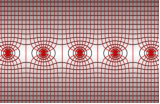
\includegraphics[scale = 2]{pictures/MWPC_electric_field.pdf} \qquad\qquad
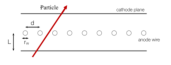
\includegraphics[scale=3]{pictures/multiwire.pdf}
\caption{Scheme for a multiwire chamber}
\label{fig:multiwire_scheme}
\end{figure}

Regarding, instead, the spatial resolution of the chambers, that is the experimental accuracy on the trace left by the particle that crossed them, it is found that this precision is inversely proportional to the distance between the wires: the nearer are the anodes, higher is the precision on the exact position of the passage of the radiation. From the point of view of the statistical analysis, the error on an eventual position measurement can be obtained, as a first approximation, using a uniform distribution between between a wire and the adjacent one ($\sigma_x = d/\sqrt{12})$), obtaining about 300 $\mu m$ for a series of anodes arranged at 1 mm distance from each other.\\
Because of the electrostatic repulsion, anyway, there is an inferior limit on the distance to which these wires can be placed, which greatly limits the accuracy of the apparatus, thank to which typical low resolutions are reached, of the order of hundreds of $\mu m$.\\


\section{Drift Chambers}
The limited resolution associated with multiwire chambers  can be strongly improved if we consider the drift time of ionization electrons too: measuring the time lapse between the production of these and their collection in the anode, and known drift velocity of the charges, $v_d$, inside the gas, a better and a more precise estimate of the position in which the radiation passed can be explicated. Just the simple relation in \ref{eq:drift_space} is needed.
\begin{equation}
\label{eq:drift_space}
x = \int^{t_d}_{t_0} v_d dt
\end{equation}
In the case that the drift speed is constant, the expression becomes linear and easier: $x = v_d\cdot t$.\\
Other type of detectors, as scintillators, can used to trigger the electronics when a particle reach the entrance of the chambers.\\

\begin{figure}[hbtp]
\centering
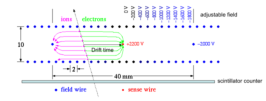
\includegraphics[scale=2]{pictures/drift_chamber_scheme.pdf}
\caption{Scheme of a drift chamber}
\label{fig:drift_chamber_scheme}
\end{figure}

The possibility to exploit these drift time allows to greatly reduce the number of wires to use, respect to multiwire detectors, or, at the same time, to further increase spatial resolution by choosing smaller spacing between wires. Considering a typical value for the drift velocity, $v_d = 5 cm/\mu s$, and a casual error on the electronic time measure of $\sigma_t = 1ns$, we obtain a spacial resolution of about $\sigma_x = v_d\cdot \sigma_t = 50 \mu m$, much smaller than the multiwire's. However, this also has a negative aspect: drift chambers exploit bigger drift length, on average, respect to others apparatus, so they are unavoidably slower and less suitable to be used in colliders (too many traces in too little time) or as trigger systems.\\
In the case of planar chambers, in which the electrons' drift occurs on the same plane in which the wires are placed, it is necessary to make sure that the speeds of the charges are fairly constant. To do that it is necessary to keep the internal electric field under control, to make it uniform and constant over time. However, as known, field lines, next to the anodes are much more it is necessary to keep the internal electric field under control. For this reason are introduced, between the anode-wires, some "potential-wires", that act like new cathodes and correct the non-uniformity of the field. \\

There are essentially four spurious effects that limit the spatial resolution of drift chambers, and their contribution is compared in the graph of figure \ref{fig:drift_resolution}:
\begin{figure}[hbtp]
\centering
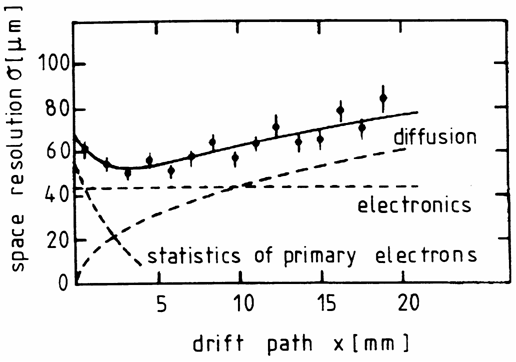
\includegraphics[scale=1]{pictures/drift_chamber_resolution.pdf}
\caption{Spatial resolution in a drift chamber as a function of the drift path}
\label{fig:drift_resolution}
\end{figure}
\begin{itemize}
\item In the case of ionization particles that cross the chamber more or less perpendicularly to it, it's important to consider the statistic production of ion-electron pairs along the trace: it is not secured that the charges are produced perfectly along the axis of the wires. This, in fact, can result in fluctuations in spatial estimates and therefore in inconsistencies in the positions of the points that will later be used to reconstruct the track. The effect is greater when the point is near to the anode, and weaker when it's far from it (the phenomenon it's schematized in figure \ref{fig:drift_ch_diff_path}).
\item Diffusion phenomena that electrons encounter as they drift towards the wire, and that affect more and more as the path of the particles increases. By integrating the diffusion equation, the contribution to the final estimate of the position to be revealed is quantified by the relation \ref{eq:diffusion}.
\begin{equation}
\label{eq:diffusion}
\sigma = \frac{1}{\sqrt{n}}\sqrt{\frac{2Dx}{\mu E}}
\end{equation}
Where $x$ is the drift distance, $D$ the diffusion constant of the gas, $\mu$ is the electrons' coefficient of mobility, $E$ is the electric field and $n$ the density of gas ions in the chamber.\\
\item The possible presence of a magnetic field affects the constancy of drift speed: as known, in the presence of the only electric field $E$, the speed with which the charges moves inside the chamber is $v_d = \frac{eE\tau}{m}$ where $m$ is the mass of the charged particle and $\tau$ its drift time. However, it shows that, with a magnetic field too, in the particular case in which this is perpendicular to $E$, the electrons tend to drift with a certain angle $\alpha$ named \textit{Lorentz angle}, calculated as:
\[ \tan(\alpha) = \omega\tau \]
where $\omega = \frac{eB}{m}$ is the cyclotron frequency of the field.\\
As can be observed in figure \ref{fig:lorentz_angle}, the drift speed too varies due to the $B$ field.\\
\item The effective electronic resolution, that can be observed especially in a delay of the start signal when the passage of the particle is detected. This contribute is fairly constant e usually limited to 1 or 2 ns, and therefore affect on the final estimate of the position only for a few tens of microns.
\end{itemize}

\begin{figure}[hbtp]
\begin{minipage}[c]{0.5\textwidth}
\centering
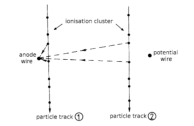
\includegraphics[scale = 2]{pictures/drift_ch_diff_paths.pdf}
\caption{Different drift paths for near\\ and distant particle}
\label{fig:drift_ch_diff_path}
\end{minipage}  
\begin{minipage}[c]{0.5\textwidth}
\centering
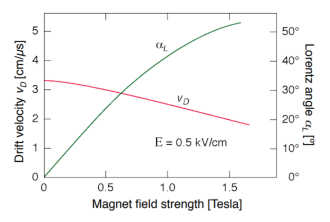
\includegraphics[scale=1]{pictures/lorentz_angle.pdf}
\caption{Lorentz angle and drift velocity in a magnetic field}
\label{fig:lorentz_angle}
\end{minipage}
\end{figure}

Another important feature associated to the drift chambers is the left-right ambiguity, that emerges when an attempt is made to estimate the distance of the particle trace from the chamber's wires.

\begin{figure}
\centering
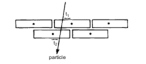
\includegraphics[width=5.5cm]{pictures/drift_ch_left_right.pdf}
\caption{Solution of the left-right ambiguity}
\label{fig:left_right_ambiguity}
\end{figure} 

The system, in fact, only measures a time interval, and therefore in no way can distinguish whether the radiation has passed to the right or to the left of the wire. Usually this ambiguity is maintained so that every hit identifies two points: one "true" (linked to the passage of the particle) and one "ghost", that will be excluded. The ambiguity can be resolved adding to the chamber many layers of cells, staggered by half a cell (as shown in \ref{fig:left_right_ambiguity}). Joining the information from the layers, it is possible to distinguish the points that actually correspond to the trace of the particle, as they are the only ones aligned, thus solving the ambiguity of the system.\\


\chapter{Muons}

\section{About the Particle}
Muons are fundamental fermions, actually classified as leptons, widely used from an experimental point of view especially thank to how they interact with matter. They have fairly higher mean lifetime than other particles, due to the fact that their decay process is mediated by the weak interaction, which timing are much larger than, for example, the strong interaction ones, of which muons don't resent. Moreover, thank to their high mass, they are less significantly decelerated in presence of electromagnetic fields, losing less energy because of effects like ionization or irradiation and penetrating even to great depths in materials they go across.\\
Another advantage brought by the experimental use of muons is that it's really easy to find them: these particles are, in fact, among the major constituents of secondary cosmic rays (so originated thank to the interaction between primary cosmic rays and Earth's atmosphere) that constantly hit the planet. In particular, the reaction responsible of the greatest production of these leptons is the following:
\[ \pi^- \to \mu^- + \bar{\nu_\mu} \qquad \pi^+ \to \mu^+ + \nu_\mu \]
In laboratory, muons can be produced in colliders, sending an high energy proton beam (\textgreater 500 MeV) versus carbon or beryllium targets, generating pions, which than decay. \\

Below are reported the official values associated to the principal characteristic of the particle.
\begin{table}[htbp]
\centering
\begin{tabular}{c c}
\toprule
\textbf{Mass} & $105.6583745(24) (MeV/c^2)$\\
\midrule
\textbf{Mean Lifetime} & $2.1969811(22) (\mu s)$\\
\midrule
\textbf{Spin} & $1/2$\\
\midrule
\textbf{Electric Charge} & $-1 (e)$\\
\midrule
\textbf{Color Charge} & $Colorless$\\
\midrule
\textbf{Antiparticle} & $\mu^+ (antimuon)$\\
\midrule
\textbf{Decay products} & $e^-,e^+,\nu_e,\bar{\nu_e}$\\
\bottomrule
\end{tabular}
\caption{Main characteristics of the muon $\mu^-$}
\label{tab:muon_parameters}
\end{table}


\section{Interactions of muons with matter}

The principal interactions 
The main interactions that the muons encounter when they go through a given material are essentially of four types:
\begin{itemize}
\item \textbf{Ionization}
\item \textbf{Bremsstrahlung}: electromagnetic radiation (i.e. a photon) produced by the deceleration of fast charged particles after the interaction with the coulomb field of a nucleus. This effect dominates for higher energy values than the critical energy, defined as the values corresponding to the configuration in which energy losses from irradiation and ionization are equal (that for the muon is estimated around 890 GeV).\\
\item \textbf{Pair production}: similar to the effect of photons, for high energy muons it can be observed that sometimes they disappearance producing a $e^+/e^-$ pair, as schematized in the reaction:
\[ \mu + nucleus \to e^+ + e^- + nucleus \]
\item \textbf{Photonuclear interactions}: for very high energy muons ( \textgreater 10 TeV), inelastic collisions muons-nucleus begin to become relevant, especially for the detectors, in which hadronic background (as hadronic jets) can be revealed.\\
\end{itemize}

\subsection{Ionization}
When charged particles, as muons, pass trough a material, lose a certain fraction of energy that they give to the electrons of the constituent atoms, due to electromagnetic interactions.\\
Such energy loss can be explicated, per unit of length, thank to Bethe-Bloch formula (\ref{eq:Bethe-Bloch}):
\begin{equation}
-\frac{dE}{dx} = \left(\frac{ze^2}{4\pi\varepsilon_0}\right)^2\frac{4\pi Z\rho N_A}{Amv^2}\left[\ln\left(\frac{2mv^2}{I}\right)-\ln(1-\beta^2)-\beta^2\right]
\label{eq:Bethe-Bloch}
\end{equation}
Where $v$ is the incident particle's speed, $z$ its charge, $\beta = v/c$, $m$ is the electron's mass, and $A,Z,\rho$ are the physical characteristic of the material. Finally, $I$ is the energy needed to ionize an atom.\\
Equation \ref{eq:Bethe-Bloch} is valid only for charged particle, with a greater mass of the electron one, and with a speed much higher than that of atomic electrons, taking into consideration that at too high speeds relativistic corrections and other types of interactions come into play. As expected, the greater part of the energy loss it's for lower velocities, when the formula goes as $\sim 1/\beta^2$ (as can be seen in figure \ref{fig:energy_loss_in_air}).\\

\begin{figure}[hbtp]
\centering
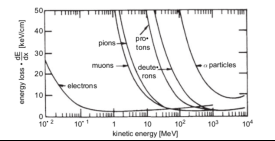
\includegraphics[scale=2]{pictures/particle_energy_loss_in_air.pdf}
\caption{Energy loss for typical particles in air}
\label{fig:energy_loss_in_air}
\end{figure}

It is to remember, however, that Bethe-Bloch's formula doesn't allow to calculate the exact energy lost by the particle, but it represents an average energy loss through a material, caused by interactions whose number must be treated in a statistical manner. This occurs especially when treating thin absorbers, in which important fluctuation of energy loss can be seen. In fact, in these case, the energy distribution is strongly asymmetric and can be represented by a Landau function.\\
Analytically:
\begin{equation}
\label{eq:landau}
L(\lambda) = \frac{1}{\sqrt{2\pi}}\exp\left[-\frac{1}{2}(\lambda+e^{-\lambda})\right]
\end{equation}
where $\lambda$ represent the standard deviation from the most probable energy lost:
\[ \lambda = \frac{\Delta E - \Delta E^W}{\xi} \]
with $\Delta E$ that is the energy effectively lost by the particle in an absorber material of thickness $x$, while $\Delta E^W$ is the most probable value predicted by the theory. Finally, $\xi$ corresponds to a series of multiplicative factors obtainable by integrating Bethe-Bloch's relation.\\

\begin{figure}[hbtp]
\centering
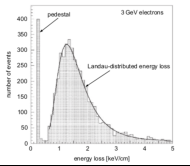
\includegraphics[width=5cm]{pictures/landau.pdf}
\caption{Energy-loss distribution of 3 GeV electrons in a thin-gap drift chamber
filled with Ar/CH 4}
\label{fig:landau_distribution}
\end{figure}

Ranges, i.e. the distance traveled within a given material by a particle before it loses all its energy, are not a problem for muons: as explained before, muons are leptons that interact very little with matter, and they do it mostly by losing energy from ionization. In the case, in particular, of cosmic muons, that are high energy particles (usually some GeV), these secondary effects are mostly negligible.\\

\begin{figure}[hbtp]
\begin{minipage}[c]{0.5\textwidth}
\centering
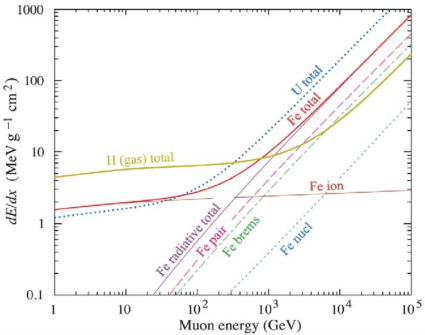
\includegraphics{pictures/muon_energy_loss.pdf}
\caption{Average energy loss of a muon in \\hydrogen, iron, and uranium as a function \\of muon energy.}
\label{fig:muon_energy_loss}
\end{minipage}  \hfill
\begin{minipage}[c]{0.5\textwidth}
\centering
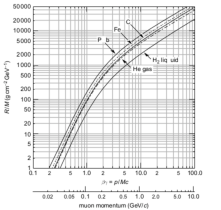
\includegraphics[scale=1.8]{pictures/muon_range.pdf}
\caption{Range of muons in liquid hydrogen, helium gas, carbon and lead}
\label{fig:muon_range}
\end{minipage}
\end{figure}

As can be seen, for example, from the line corresponding to gaseous hydrogen, in figure \ref{fig:muon_energy_loss}, up to a few hundred GeV, the only significant effect that contributes to slowing down the muons is ionization.\\



\part{LEMMA}

\chapter{Experimental setup}
\label{ch:exp_setup}

\section{LEMMA}
The experiment was born within the LEMMA project (which stand for Low Emittance Muon Accelerator), that consists in a particular type of approach developed in recent years for the study of these particles.\\
As known, the utility of muon colliders in the development of new physics is really high: first of all, differently to other elementary particles (for example to the protons) they are less interactive, so in a muon beam all the energy and the momentum are available, in absence of subsystems interaction; moreover, the greater mass respect to other used particles reduce the energy loss for synchrotron radiation.\\
However, a problem exists in the beams production. Muons are usually produced in high energy hadrons collisions on a target, but with this method the obtained beams have too high emittance, made by low localized particles, much to need a cooling phase, before using them. The problem is that this cooling process requires a certain period of time, during which muons tend to decay.\\
A low emittance particle beam, is a beam in which all the particles are confined to small distances between each other, and all of them have more or less the same momentum, so that it can already be used in a collider or in an accumulation ring \cite{bib:low_emittance_muon_collider}. A low emittance beam can be obtained sending positrons on a target, and taking advantage of their annihilation on target's electrons at rest. The main benefit of this solution is that $\mu^+/\mu^-$ pairs produced are confined in a in a very restricted spatial region, limited both longitudinally and transversely.\\
To summarize, LEMMA project \cite{bib:LEMMA} allows the construction of low emittance muon beams, spatially delimited, that don't need a cooling phase and that allow operations at very high center of mass energy. All this allow to work with an high collection efficiency (less muon decaying) and a lower background events number, at the expense of a lower cross-section, that implies less muons produced respect to other techniques.\\


\section{Test beam setup}
Experimental setup consists in four drift chambers, a revisited version of the ones used in CMS to detect muons. The system has been reproduced at Legnaro in 2018, and it is actually used to collect data for cosmic muon's tracks reconstruction.\\
The project was initially born as a test beam, to study muon bunches and valuating their main physical characteristic, to determine if they were ready to be used in a collider. In particular, it was used to analyze $\mu^+/\mu^-$  pair production after the collision of a 45 GeV positron beam on a Beryllium target.\\
The scheme of the first apparatus built (2018) is reported in figure \ref{fig:lemma_test_beam_2018}, of which the four drift chambers are only the final part (light blue lines).\\

\begin{figure}[hbtp]
\centering
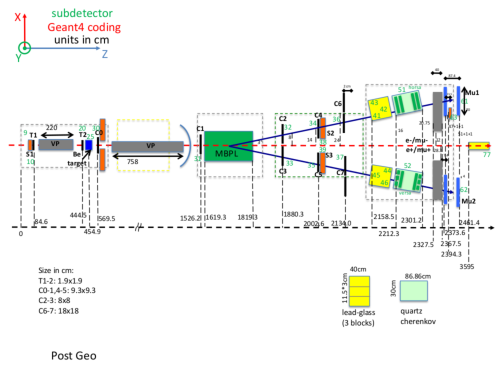
\includegraphics[width=\textwidth,height=0.4\textheight]{pictures/lemma_2018.pdf}
\caption{Experimental setup used for test beam in 2018}
\label{fig:lemma_test_beam_2018}
\end{figure}
 Regarding the chambers, each of them is built consists of four layers of drift tubes, which each contains 16 cells (42 x 13 mm) in the center of which a metallic wire act as an anode, while cell's border work as a cathode. The electric field inside the cell goes as $1/r$, where $r$ is the distance from the center, and therefore attracts ionization electrons produced after the passage of a muon through the gas contained in the detector ( $85\%$ Ar and $15\%$ CO\textsubscript{2}). As the drift velocity of the electrons in the gas is constant, it is possible, thank to an electronic system that measure the arriving time of the first ionization, to reconstruct the exact position (respect to the center) in which the muon passed, but with a left-right ambiguity as seen before in \ref{fig:left_right_ambiguity}. Combining the information of three or four consecutive cells belonging to different layers, it is possible to resolve this ambiguity and to reconstruct the local passage of the particle; then, knowing the points that compose that local trace, it's not difficult to process the global one, which actually delimits the path of the muon through the chambers. An example of a track reconstructed, that comes from a 2018 calibration file (made by data collected by sending single muons produced expressly to calibrate the apparatus), it is reported in figure \ref{fig:example_track_2018}.\\

\begin{figure}[hbtp]
\centering
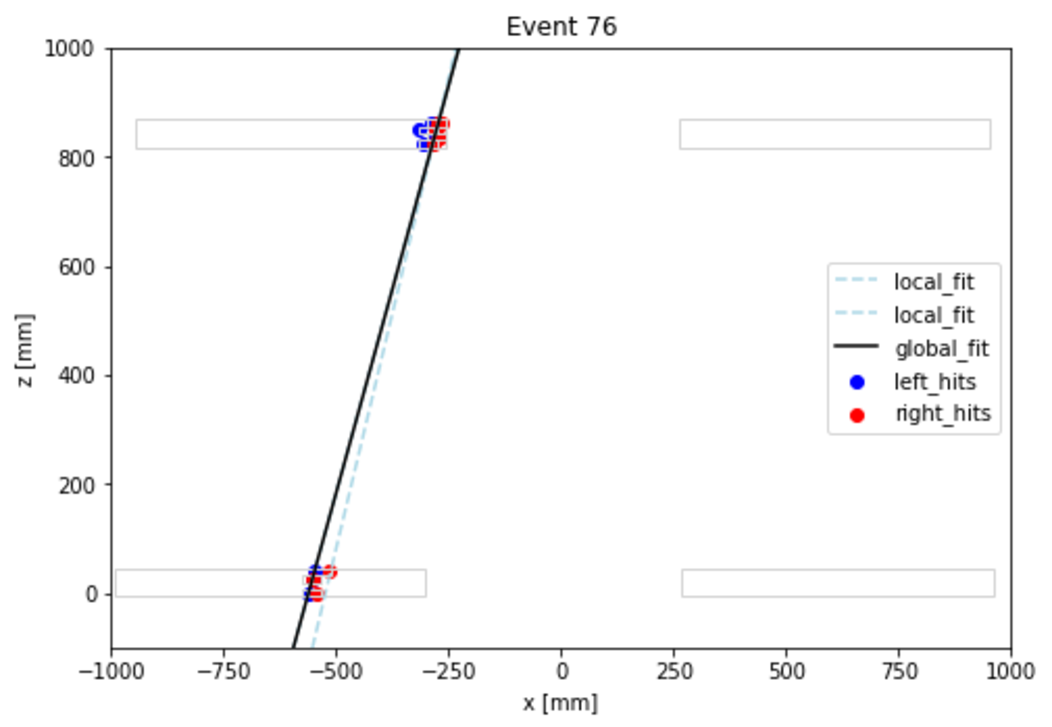
\includegraphics[scale=0.4]{pictures/2D_example_global.pdf}\hfill
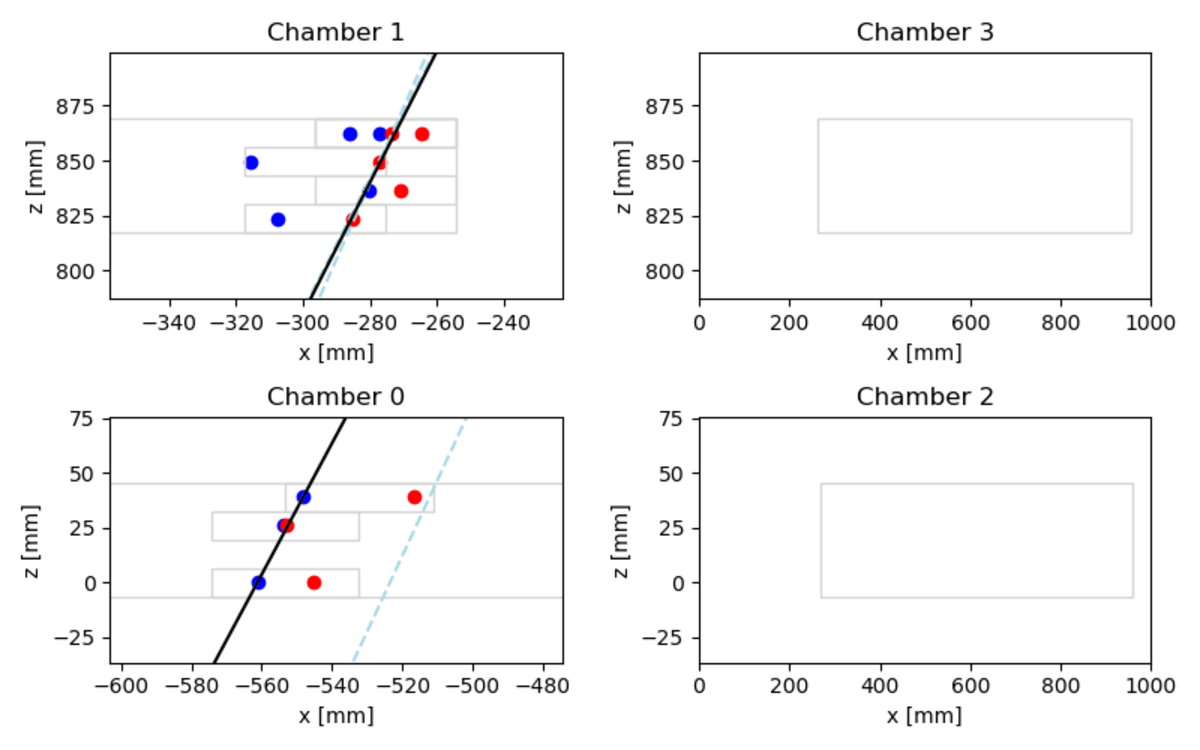
\includegraphics[scale=0.4]{pictures/2D_example_chambers.pdf}
\caption{Track recostruction in 2-dimensional setup (2018)}
\label{fig:example_track_2018}
\end{figure}

The example displayed in figure \ref{fig:example_track_2018} its a quite "clean" event, in the sense that it doesn't show other signal, expected the one used for the interpolation, which unfortunately does not happen often.\\
Note that, as in most of the events, local and global tracks don't coincide perfectly: the cause lies both on imprecision of the acquiring system and on sensibility issues of involved instruments. It is not to forget, then, that drift tubes do not provide information on the three-dimensional position in the wire direction.\\


\subsection{Trigger and trigger-less data aquisition}

Data are collected thank to an electronic system that read detector's sensor at 40 MHz (i.e. every 25 ns), without the need of an external trigger, and register them every time that at least one hit has been revealed in one cell. It will be a task of the algorithm to distinguish between signal hits and background hits, due to noise in the electronics.\\
There is also a hardware device in the system that  has implemented a mean time firmware that automatically try to recognize partial alignment in the cells, and launches a signal similar to that of a trigger, marking as "probably good" the event in which it has spotted that alignment.\\
The electronic system register raw data in hexadecimal format and produce a csv file. Every raw of the file is encoded in the same way, with six fields that identify unambiguously the hit described and allow to go back to the position of passage of the particle.\\
For reasons that still are not well understood, the experiments done with this setup (but for next ones too) are characterized by an intense noise, of a purely electronic nature, understood as a big number of background signals in the data. For this reason the algorithm that analyze collected data should be little sensitive to noise, so much selective in the identification of signal events.\\
The first reason behind the choice of not installing an external trigger lies precisely in the high noise that characterizes these chambers: trying to directly find an alignment allow, in fact, to work only to "clean" events, at the expense of an high efficiency (defined as the ratio between the number of muon revealed and of the particles that effectively passed through the detector).\\



\subsection{Cosmic muon setup}

Actually (2019), the instrumental apparatus has been repositioned turning the chambers upwards, in order to detect cosmic muons. The principles of operation are exactly the same, as the electronic system: only the geometry of the problem has been changed, and now allows the three dimensional reconstruction of the tracks. The four chambers are now arranged one above the other (as in figure \ref{fig:2019_esp_setup}), parallel to two by two, so that a couple of detectors will register the information in the $x$ direction, while the other couple in the $y$ direction ($z$ axis is the vertical one, the direction where the muons come from).
\begin{figure}[!hbtp]
\centering
\includegraphics[scale=0.06]{pictures/2019_setup.pdf}
\caption{2019 Experimental setup to spot cosmic muons}
\label{fig:2019_esp_setup}
\end{figure}

The flexibility of the apparatus, however, doesn't prevent the installation of a real trigger system: recently, in fact, a couple of scintillators has been installed (figure \ref{fig:2019_esp_setup_2}). The advantage brought by these is the high efficiency with which they are able to detect the passage of a muon (next to 100\%), at the expense of selectivity. Moreover, we must take into account that the surface of these new implemented devices is lower respect to chambers one (about 1/4), so they do not cover all the effective volume.\\
The principal utility of the scintillators resides in the search for a better efficiency and in the possibility to have a comparison with data collected thank to the mean timer firmware.\\

\begin{figure}[!hbtp]
\centering
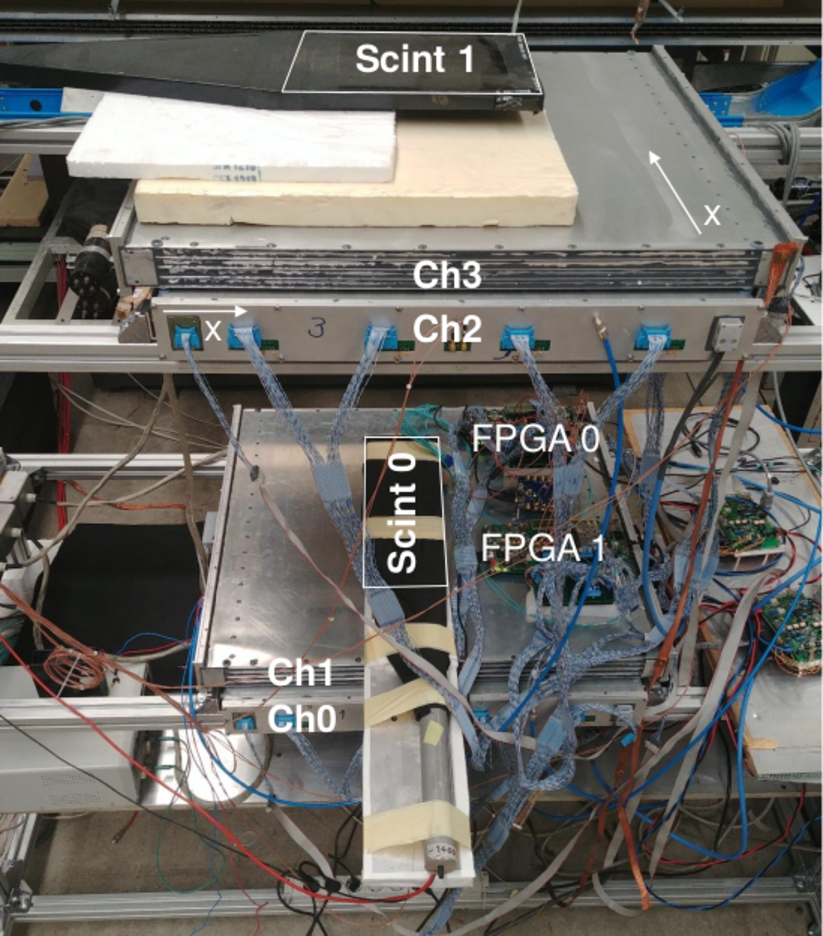
\includegraphics[scale=0.5]{pictures/2019_scint.pdf}
\caption{2019 Experimental setup to spot cosmic muons}
\label{fig:2019_esp_setup_2}
\end{figure}


However, the data elaborated in this thesis have been collected before the installation of the scintillators, and they will be filtered and analyzed with a \textit{triggerless} method, through an appropriate algorithm.\\



\chapter{Preprocessing and raw data analysis}

The electronic system currently in use, registers the signals from the detectors, and writes them to a csv file: hits contained in this are encoded through six fields (HEAD, FPGA, TDC\_CHANNEL, ORB\_CNT, BX, TDC\_MEAS), that allow to uniquely identify the chamber, the layer and the cell in which the signal has been revealed. Then, thank to a simple equation (written in \ref{eq:TIME-NS}), it is possible to compute the time taken by the ionization electrons to reach the anode.
\begin{equation}
t = ORB\_CNT\cdot3564\cdot25+BX\cdot25+TDC\_MEAS\cdot25/30
\label{eq:TIME-NS}
\end{equation}
Actually, having not yet developed an online analysis method, the system simply saves files of raw data until they reach 10 MB in size.\\
These files are first processed by the algorithm, that optimizes occupied memory (like removing redundant information as the HEAD field in the csv file, that is the same for all the hits), reconstruct the events and elaborates a first and more superficial selection.\\
From this first processing phase is produced a new file, that contains all the "accepted" signals, grouped by events (based on collection absolute time), ready to be passed to the second part of the program and, in particular, to the track reconstruction.\\

\begin{footnotesize}
Actually the algorithm manages the triggerless analysis of the hits, but let a first selection exploiting the meantimer already implemented in the electronic system. This one, but any external trigger too, marks the hits that they recognize as belonging to signal events with a 64 bit special sequence (a row in the csv file) containing the information related to the trigger. At the time of data capture the only active system was, precisely, the meantimer, identified in the file by the TDC\_CHANNEL (= 139) field.\\
The algorithm, as mentioned above, does not provide for particular actions for the hits marked by external triggers (but for the 139), except for a first selection, but foresees the possibility.\\
\end{footnotesize}


\section{Recostruction of the events}

The first (and easier) step is to "complete" the dataframe containing all the hits, adding the necessary information to allow a more intuitive view of the problem, and replacing fields generated by preprocessing phase with more useful parameters like the index of the chamber, the layer and the precise cell in which the hit has been revealed. It is important too to compute (as seen in \ref{eq:TIME-NS}) the time elapsed between the actual passage of the particle and the electronic signal reception (later we will see that this estimate needs to be corrected).\\
 It is precisely this temporal value that allow grouping hits into complete signal events: cosmic muons come to earth with very high speeds (estimated around 30 cm/ns \cite{bib:cosmic_muons}), and therefore, to travel across one of the detectors (not more than 6/7 cm thick) they only take a few fractions of a nanosecond, a much shorter time than the one used to collect ionization electrons. As far as these are concerned, in fact, it is known the drift velocity inside the gas of which the cells are full, and therefore, knowing cell's length, you can obtain another important parameter for this system: the maximum drift time needed to collect all the electrons (especially those produced on cell's border), that is estimated around 390 ns.\\
Thank to this $T_{MAX}$ it is possible to group temporally the hits, letting the electronic system catches charges those are produced far away from the anode too. From a technical point of view, this request consist in asking for consecutive hits in the dataframe which are temporally distant, among themselves, less than the 110\% of the maximum drift time (not 100\% to take into account the accuracy of used clocks), to be part of the same event.\\
Such a discriminating factor is necessary: if the electronics read detectors every 25 ns, one cannot hope to have gathered all the charge in such a sort period of time, but has to merge the information collected on multiple acquisitions.\\
Lastly, a first condition on these newly built events is imposed: they need to consists in at least six different hits, or they will be immediately drop out. The motivation resides in the high presence (emerged looking on raw data preprocessed files) of background events, made by only one or two signals, that are useless for the next analysis and don't represent nothing physical. Also, six is the minimum number of hits which will be requested later for a global linear fit.\\


\section{Time Pedestal}

The next step consist in the computing of the exact distance from the wire to which muons passed, calculable knowing the drift time of the electrons produced during ionization, using the relation \ref{eq:POSITION}:
\begin{equation}
x = v_d\cdot(t-t_0)
\label{eq:POSITION}
\end{equation}
Where $t_0$ is an appropriate parameter, called time pedestal, that contains contributions due to trigger latency (absent in this case) and due to the time necessary for the electronics to detect and collect data \cite{bib:CMS}. The drift speed $v_d$, instead, it is assumed constant inside the cell.\\
Any corrections to these two parameters will be made during the calibration phase.\\
In an ideal detector, the temporal measurements of the signals collected would follow a uniform distribution from 0 ns (corresponding to the passage of the muon next to the anode) and 390 ns (passage on cell's border). In practice, however, there are inevitable delays in the signals due to trigger latency or simply due to length of front-end electronic cables, that contribute to the measured time (TIME\_NS)  as follow:
\[ TIME\_NS = t_{drift} + t_{wire} + t_{trigger} \]
These secondary contributions are usually corrected by calibration tests or analysis of time distributions, readjusting the measures so that they follow the expected uniform distribution.\\
Another benefit related to the use of such a structure of detectors placed one above the other is the possibility to exploit the geometry of the system, in particular the disposition with which the layers (made by cells) have been installed, to explicit a set of mean timer equations (thank to Talete's theorem) that let you to compute the time pedestal of the detector directly during the construction of the events.\\
From a pratical point of view, the theorem is applicable on appropriate alignment patterns in the disposition of the signals inside the chambers, an example of which is represented below, in figure \ref{fig:alignment_pattern}, and it is resolved by equation \ref{eq:t0_pattern} (in which every measured time $t_i$ is defined less than a constant, $t_i = t_i + t_0$, that is the same for every point), where $T_{MAX}$ is the maximum time interval in which all the ionization charge has been collected, that is estimated at 390 ns.
\begin{figure}[hbtp]
\begin{minipage}[c]{0.5\textwidth}
\centering
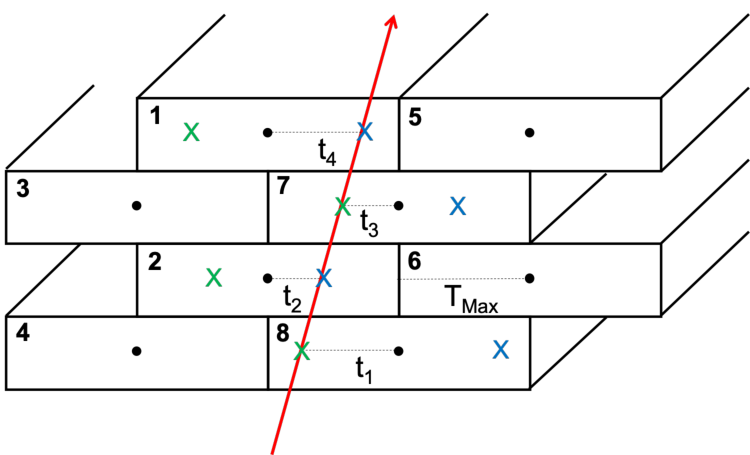
\includegraphics[scale=0.5]{pictures/scheme_track_chamber.pdf}
\caption{Possible pattern for a mean timer equation}
\label{fig:alignment_pattern}
\end{minipage}  
\begin{minipage}[c]{0.5\textwidth}
\begin{align}
&T_{MAX} = \frac{t_1+t_3}{2} + t_2 = \frac{(t_1 + t_0) + (t_3 + t_0)}{2} + (t_2 + t_0) \nonumber \\
& \nonumber\\
&t_0 = \frac{t_1 + t_3 + 2\cdot t_2 - 2\cdot T_{MAX}}{4} \label{eq:t0_pattern}
\end{align}
\end{minipage}
\end{figure}

In reality, each cell should have its own $t_0$, but the differences between the values are of the order of a few ns at most, so they are negligible, in first approximation. For this reason the algorithm proceeds in this way:
\begin{itemize}
\item[-] Data are grouped in single events, and it is made a first selection, dropping out every event that is made by less than two chambers that contain at least 3 different layers of hits (i.e. the minimum configuration to build, afterwards, a track).
\item[-] Single event is taken, and the hits it's composed to are further divided by chamber, and passed to the real mean timer algorithm.
\item[-] Without entering too much into the technical, the algorithm combines the cells in the chamber, in which the signal has been revealed, in every possible combination of three elements, and finds the triplets to which it is possible to apply Talete's theorem, calculating the relative time pedestal by resolving a mean timer equation similar to the one written in \ref{eq:t0_pattern}.
\item[-] In the case (fairly frequent) that in the same chamber more solvable patterns appear, the algorithm computes all the possible estimates for $t_0$ and simply takes the mean as final value.
\item[-] The estimate (or eventually the mean of the computed values) thus found of the time pedestal it is extended to all the hits that are part of one of the alignments found by the program, allowing a correct valuation of their actual drift time. It is useless to specify that all the points that don't belong to any alignment pattern are directly excluded by the dataframe.
\end{itemize}

Known, at this point, the correct drift time for the electrons for every single hit, it is trivial to calculate the horizontal coordinate of the passage of the muon, with the cinematic relation $x = v_d(t - t_0)$ (with $v_d$ drift velocity of the ionization charges in the gas and $t$ temporal measurement of electronics). It is important to remember that left-right ambiguity is still unresolved, and and that therefore the $x$ coordinate just found will determine two points in the cell, and not only one.\\
A last selection is made removing hits with an unphysical position value, i.e. the points that appear "outside the cell" (cell in which they were found), with a $x$ value lower than 0 or greater than 21 mm (length of half a cell).\\
At this point the efficiency of the method can be checked, for example looking at time distributions after the measurement and after the time pedestal correction. It is expected a uniform distribution between 0 and 390 ns, i.e. the limit values according to cell's dimension and electrons' drift speed.\\ 

\begin{figure}[hbtp]
\begin{minipage}[c]{0.5\textwidth}
\centering
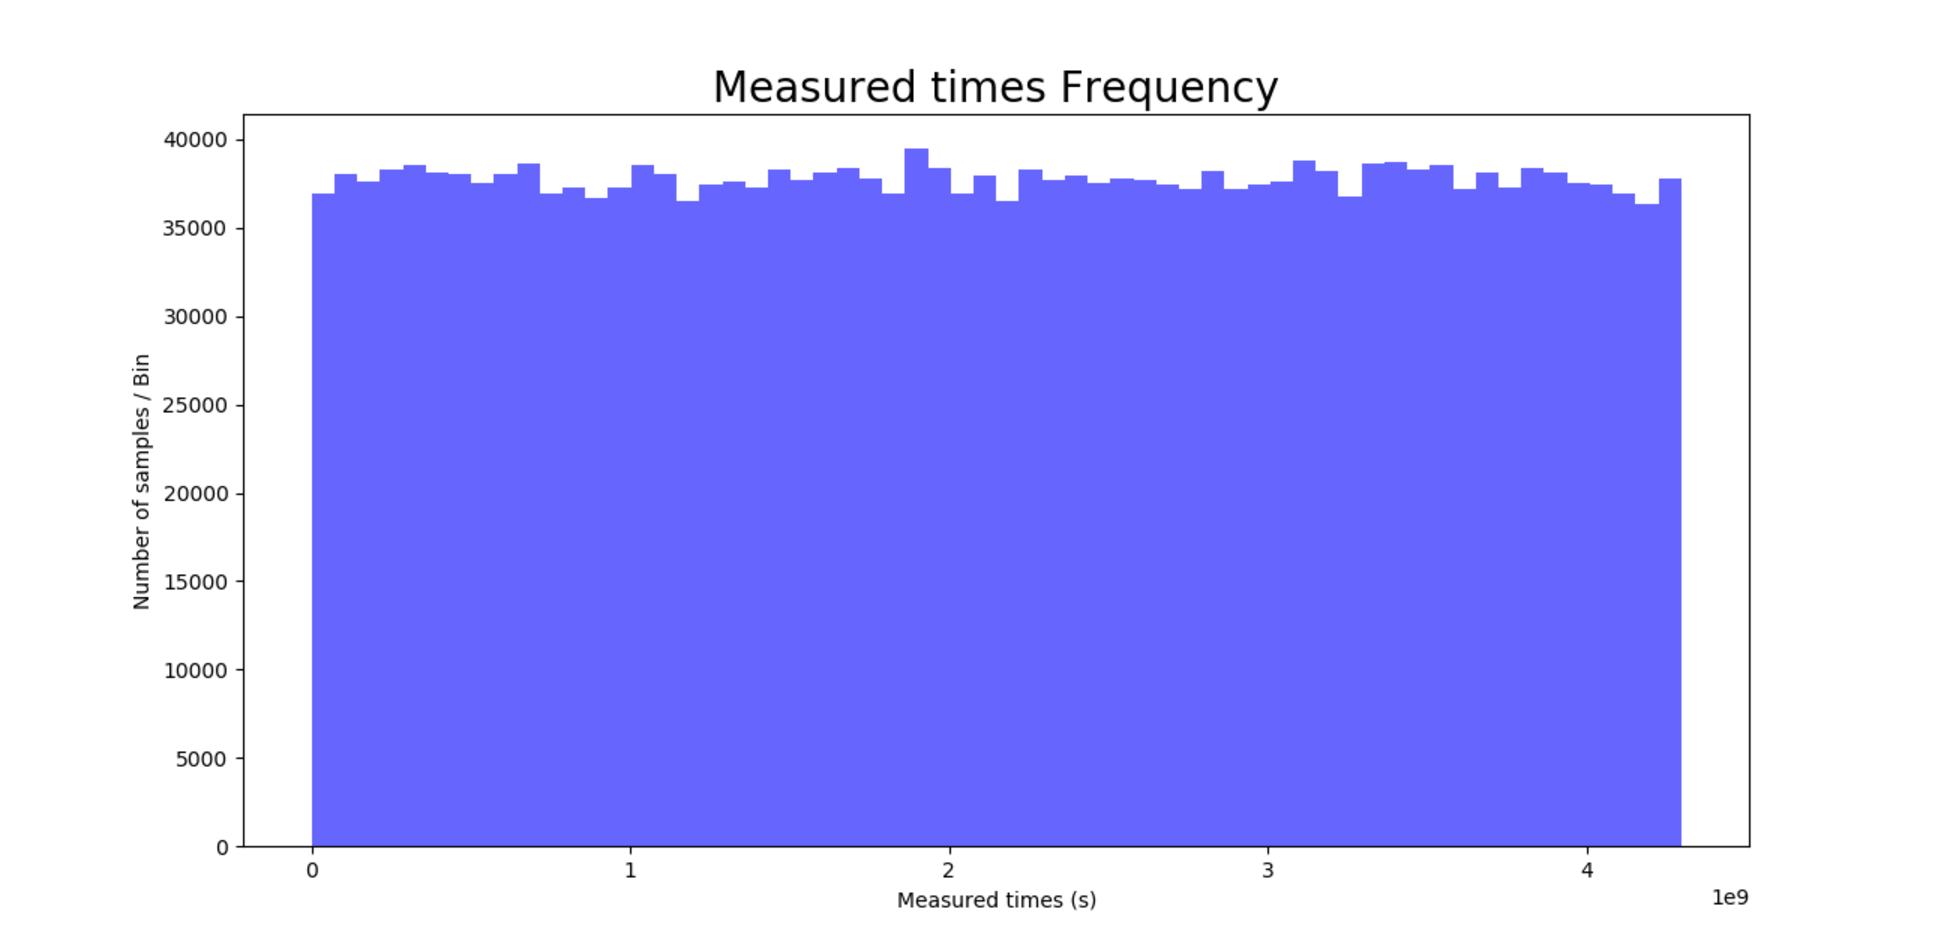
\includegraphics[scale=0.25]{pictures/Measured_times_Frequency.pdf}
\caption{Distribution of measured drift times}
\label{fig:TIME_NS}
\end{minipage}  
\begin{minipage}[c]{0.5\textwidth}
\centering
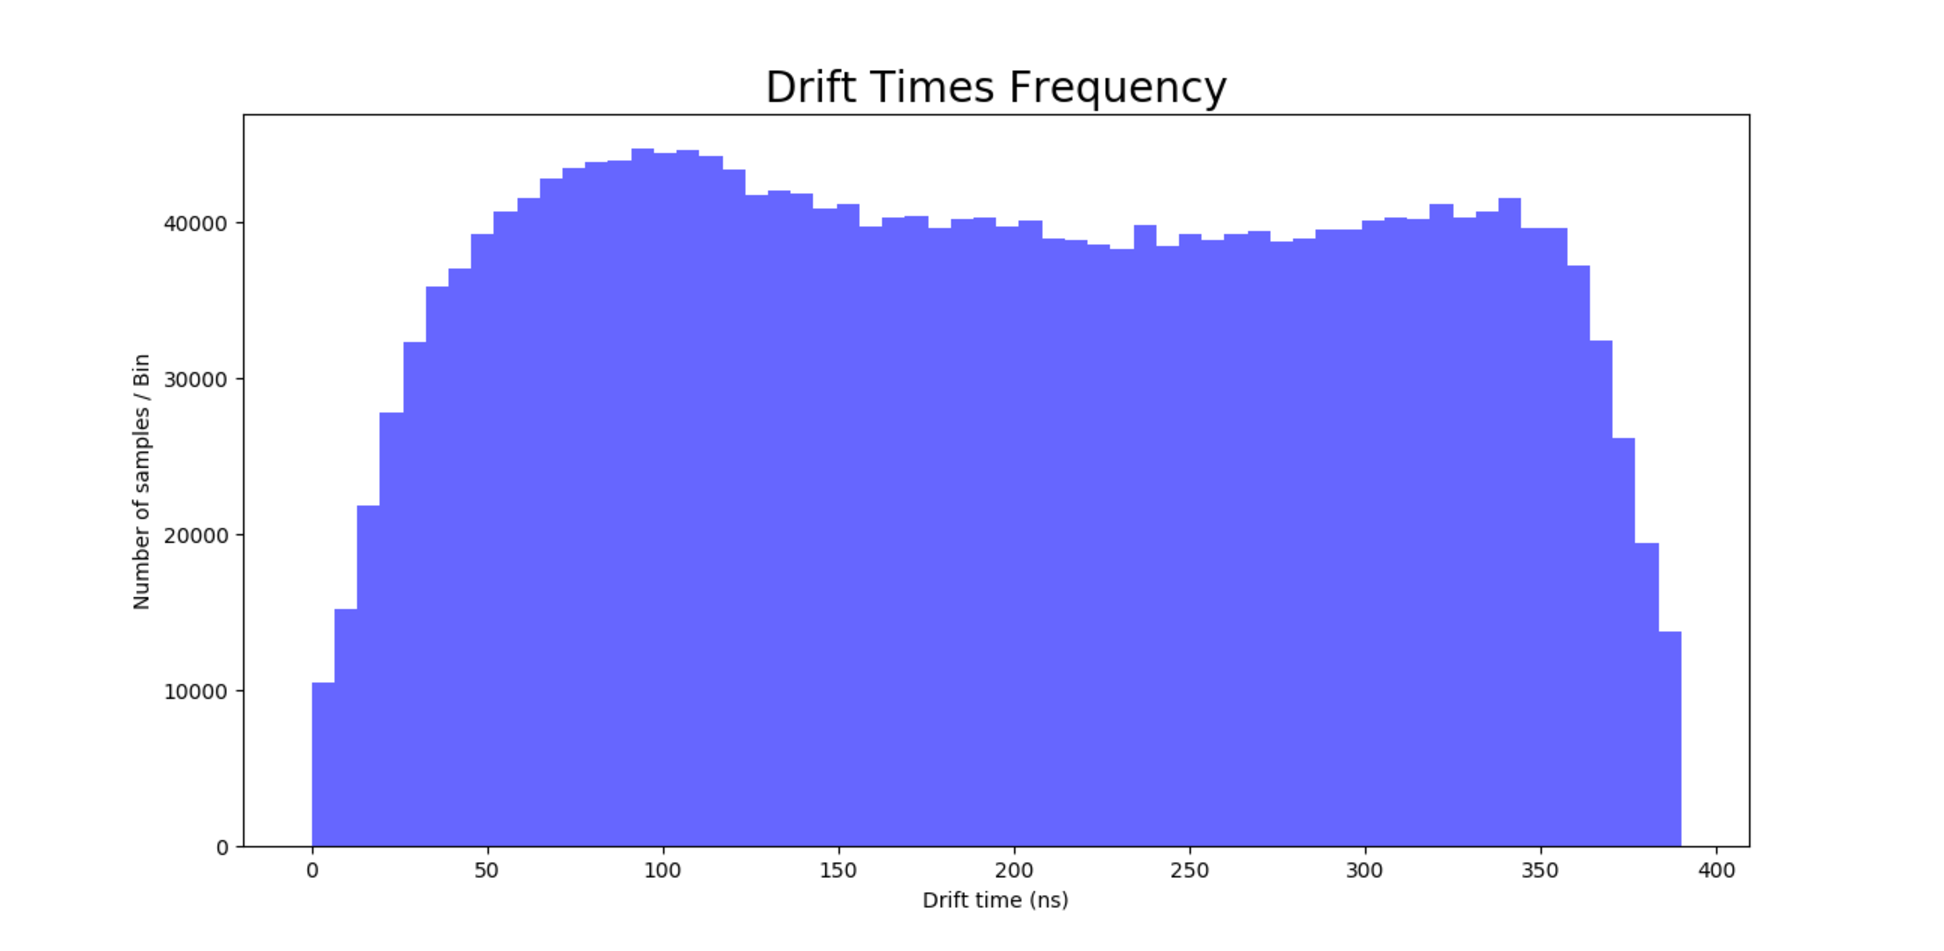
\includegraphics[scale=0.25]{pictures/Drift_Times_Frequency.pdf}
\caption{Final distribution of drift times}
\label{fig:DRIFT_TIMES}
\end{minipage}
\end{figure}

Regarding the measurements, the results are consistent with expectations; moreover, we can see how the distribution is uniform between 0 and a little more than 400 ns, concrete sign of the contribution due to this time pedestal. Regarding, instead, the effective drift times, the distribution has obvious irregularities, that can be traced to various reasons, as the effect that ionization electrons encounter depending on where they are produced (described in \ref{fig:drift_ch_diff_path}). Another possible reason is due to the way that the algorithm processes drift times: if many alignment patterns are present in the chamber, in fact, only the average value of the time pedestal found is taken into account (and we are not even sure that these values were compatible).\\
So, all these reasons could have caused the spurious effects observed in the graph, that however, in the aftermath, is not such a bad distribution for the problem.\\
However, the method used remains quite efficient, and the achieved results will then be subjected to a calibration phase to try to eliminate the anomalies.\\


\section{Raw data analysis}

There are many possible analysis to do for collected data, even before starting to reconstruct the traces, even before the calibration of the system. These preliminary analysis, in general, however, are not used to study muon's physical characteristics, but for first estimate of the efficiency of the algorithm and the functionality of the various instruments, as well as an a priori classification of the events we will be dealing with.\\
First, the efficiency of all the used selection method's (and, in general, of the mean timer algorithm) can be quantified: table \ref{tab:trigger_efficiency} reveals that about the 90\% of the collected signals belong to background events. One could be led to think that the cause of this is a too selective algorithm but, as explained above, the code simply checks the existence of alignment patterns and excludes the events for which a bad value for the drift time is found. So the program doesn't delete noisy events, but only the isolated signals. The wording "shower" that appear in the table, also, is referred to those "muon showers" of particles that may originate in the detectors, and are made by a large number of signals in various chambers. These events unavoidably show many alignment triplets (there are so many hits, in fact, that almost all the cells in a certain region are marked), so they are easily accepted by this first part of the code; it is impossible, however, to distinguish inside them complete tracks.
\begin{table}[htbp]
\centering
\begin{tabular}{c|c}
\toprule
\textit{Total hits detected (signal + background)} & 24494976\\
\midrule
\textit{Total events identified} & 66543\\
\midrule
\textit{Total hits belonging to identified events} & 2265046 (9.25 \%)\\
\midrule
\textit{Showers ( \textgreater 20 hits)} & 1621 (0.60 \%)\\
\midrule
\textit{Showers ( \textgreater 40 hits)} & 139 (0.05 \%)\\
\bottomrule
\end{tabular}
\caption{Selection efficiency of the algorithm}
\label{tab:trigger_efficiency}
\end{table}
Another useful study emerges evaluating single cell's efficiency: in the picture \ref{fig:hit_freq} is represented a two-dimensional graph, containing information on the quantity of (accepted) signals spotted by every single cell. The first thing to notice are many dark cells in chamber 0: the cause is known and resides in problems of a mechanical nature. In fact chamber 0 was the first to be installed, 
and later it was noticed that some cells were deactivated, and not able to collect signals. However, considered a useless effort to disassemble it (it is the lower-lying chamber, so it would be necessary to disassemble the entire apparatus), only a few cells are seriously damaged, so this problem does not affect the final results very much. The darker zones around damaged cells, instead, are a consequence of the mean timer algorithm: since there are no signals in some cells, the program is forced to exclude every pattern that involves these ones. Lastly, a small region of inefficiency should be noticed in chamber 1, denoting the existence of  some partial screen effect which limits the passage of particles in that area.\\

\begin{figure}[!hbtp]
\centering
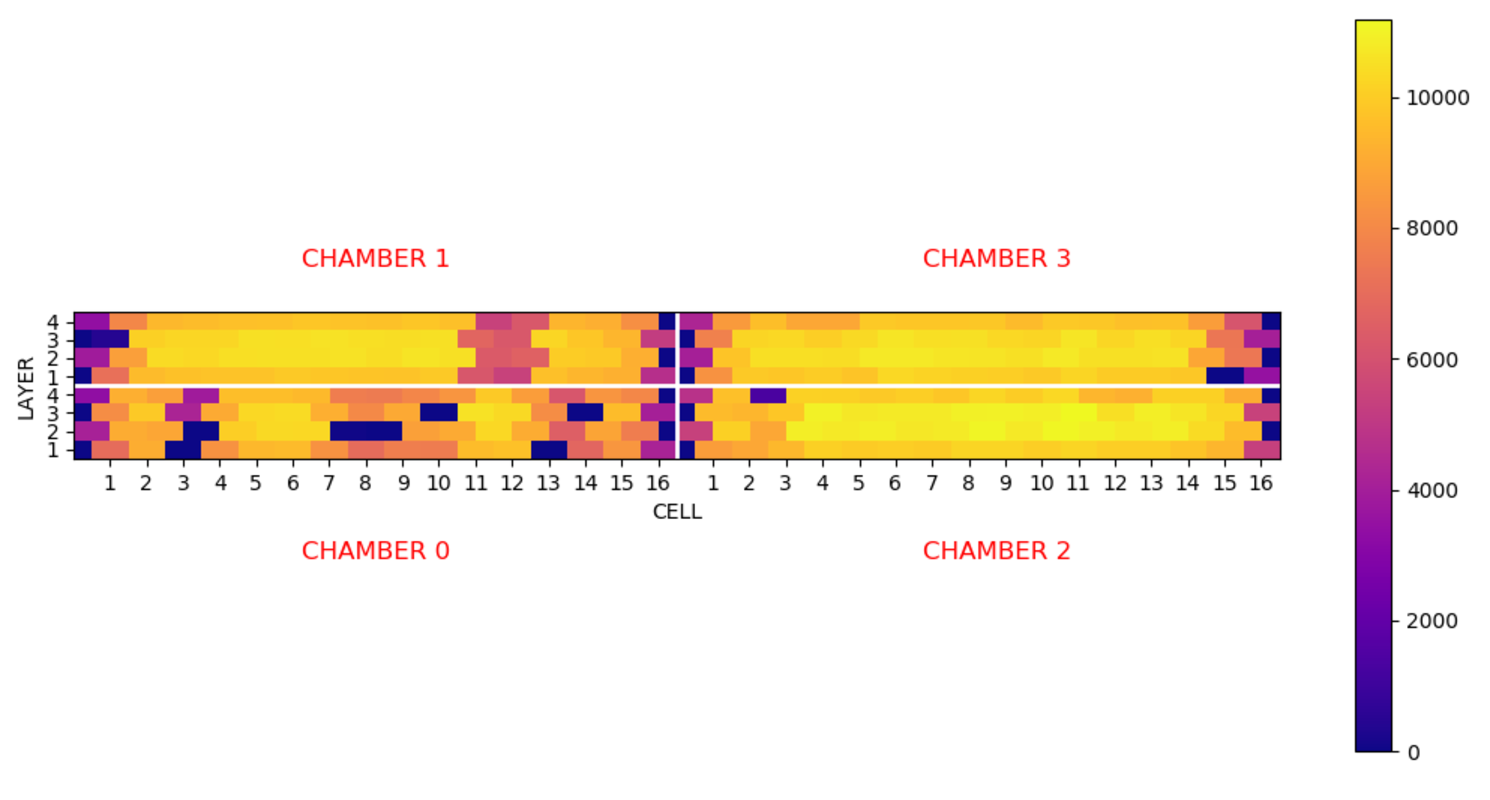
\includegraphics[scale=0.7]{pictures/Hit_matrix.pdf}
\caption{2D representation of hit frequency in the cells}
\label{fig:hit_freq}
\end{figure}

The next useful instrument to valuate chambers efficiency can be the two-dimensional plot of the relative number of signals present between the detector pairs (reported in the figures \ref{fig:ch1_ch0}, \ref{fig:ch1_ch0_zoom} and \ref{fig:ch3_ch2}). As can be seen in the zoomed picture, most of the events are made by less than 10 hits for chamber, and many peaks can be noticed at the values of 3 and 4 hits (in both chambers, but also for only one) that correspond to a signal event, i.e. the actual passage of a particle. Anyhow, events made by a large number of hits (those that in table \ref{tab:trigger_efficiency} were classified as showers) are not absent.\\

\begin{figure}[!hbtp]
\begin{minipage}[c]{0.5\textwidth}
\centering
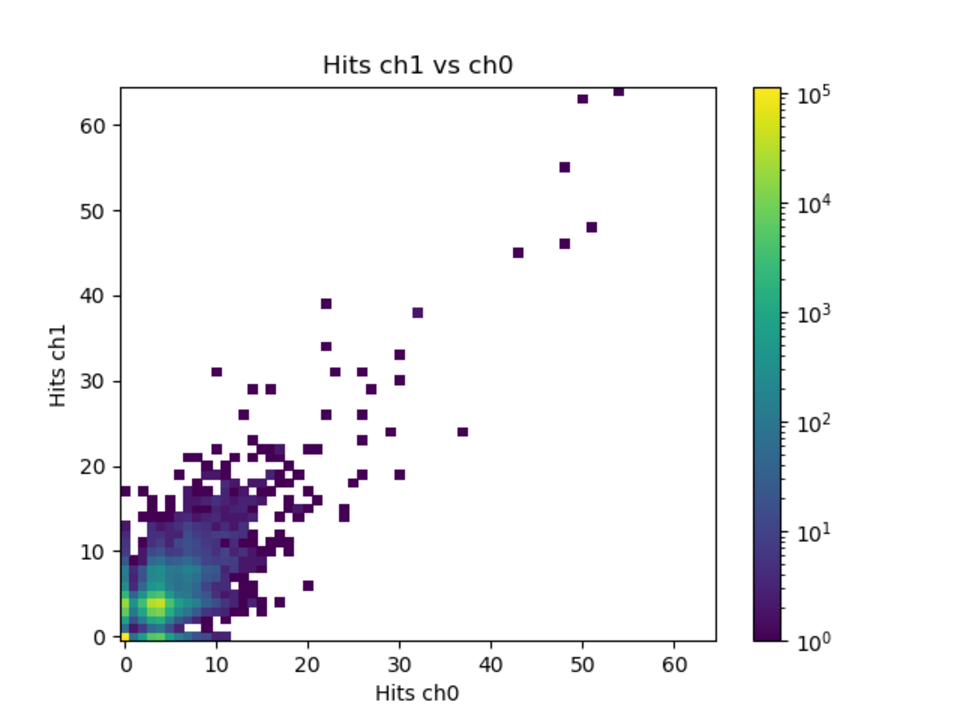
\includegraphics[scale=0.5]{pictures/Hits_ch1_vs_ch0.pdf}
\caption{Hits distribution between chamber 0 and 1}
\label{fig:ch1_ch0}
\end{minipage}  
\begin{minipage}[c]{0.5\textwidth}
\centering
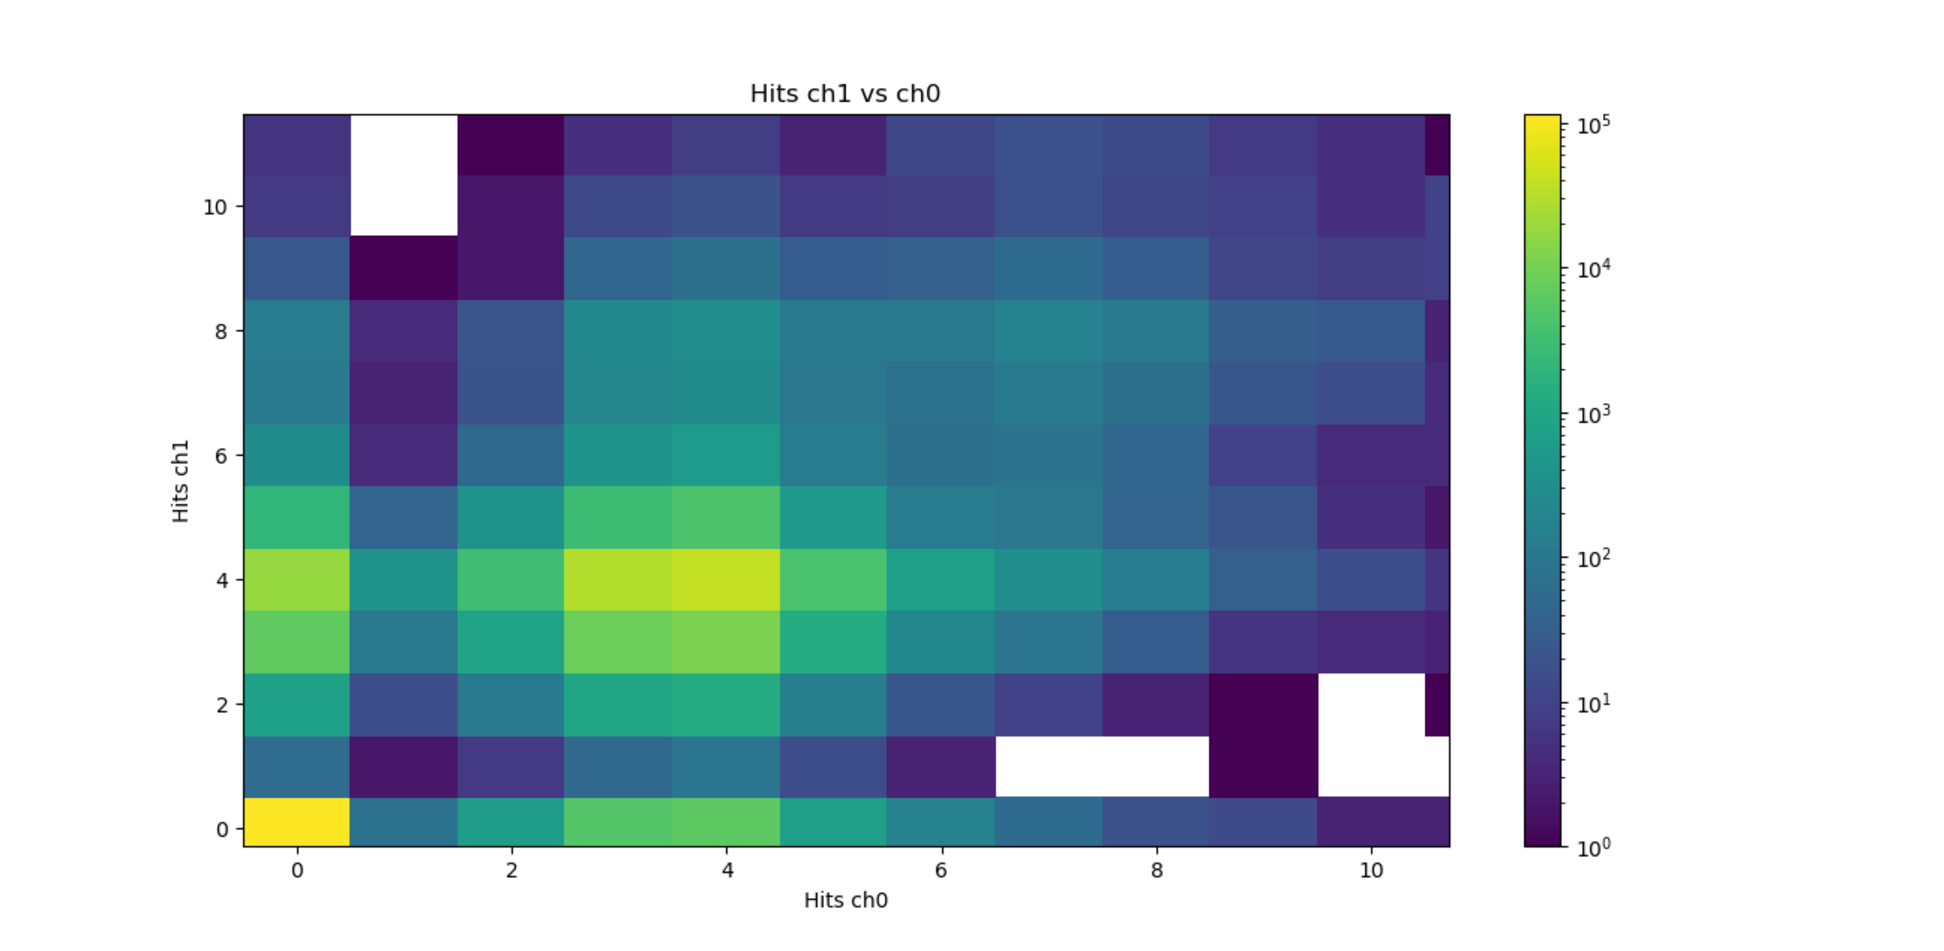
\includegraphics[scale=0.3]{pictures/Hits_ch1_vs_ch0_zoom.pdf}
\caption{Zoomed on events with 10- hits}
\label{fig:ch1_ch0_zoom}
\end{minipage}
\end{figure}

The same operation can be repeated to valuate the FPGA efficiency too (figura \ref{fig:fpga0_fpga1}). Immediately, the same features of the chambers' graphs can be noticed: the various peaks still represent a good number of signals (3 or 4 for chamber that become 7 or 8 in the FPGA) as each of these two devices "looks" for a couple of chambers (one above the apparatus and one below it).\\

\begin{figure}[hbtp]
\begin{minipage}[c]{0.5\textwidth}
\centering
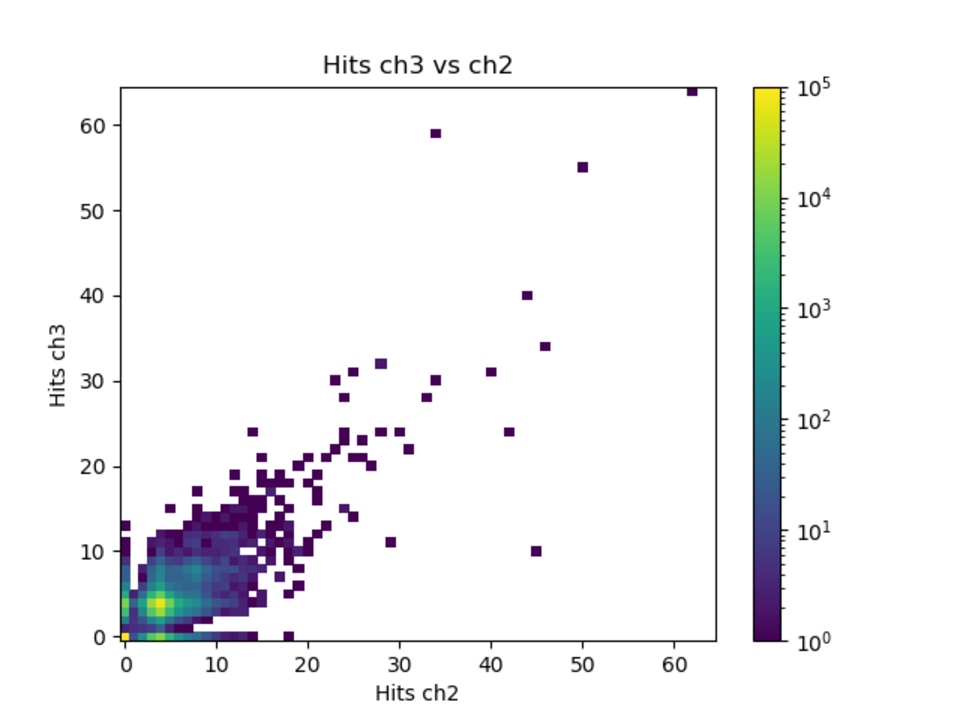
\includegraphics[scale=0.5]{pictures/Hits_ch3_vs_ch2.pdf}
\caption{Hits distribution between chamber 2 and 3}
\label{fig:ch3_ch2}
\end{minipage}  
\begin{minipage}[c]{0.5\textwidth}
\centering
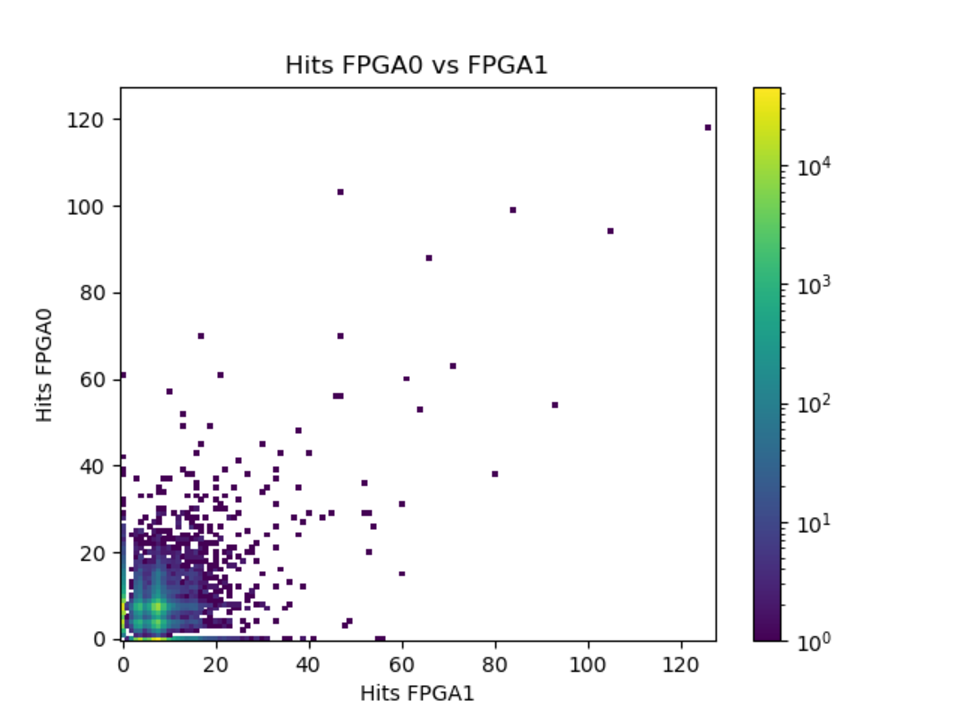
\includegraphics[scale=0.5]{pictures/Hits_FPGA0_vs_FPGA1.pdf}
\caption{Hits distribution between FPGA 0 and 1}
\label{fig:fpga0_fpga1}
\end{minipage}
\end{figure}

So far there has always been talk of a "good" number of hits per chamber (at least one per layer), corresponding to the minimum number of points needed to reconstruct at least a local track. As can be seen from the graph \ref{fig:hits_per_event} (from which too noisy points has been excluded), most of the events selected by mean timer looks "good", or at least has a good number of alignments. The higher column (8 hits), in fact, represents a signal event, since 4 points in two different chambers (one above and one below) constitute a trace or, at least, its projection on one of the two plans (xz or yz). There are events even more beautiful, that show about 15 or 16 hits: in the best case these hits are divided into 4 per chamber, which allows to reconstruct the passage of the muon in 3 dimensions.
The peak at 4 hits, instead, is due to the work method of the mean timer algorithm: probably, an alignment in one of the chambers has been revealed (so the event has however been reconstructed), but the signals in the others were excluded, probably because of a missing alignment, or an error in the compute of the position of the hits (due to some approsimations), or a wrong estimate of the time pedestal.\\

\begin{figure}[hbtp]
\centering
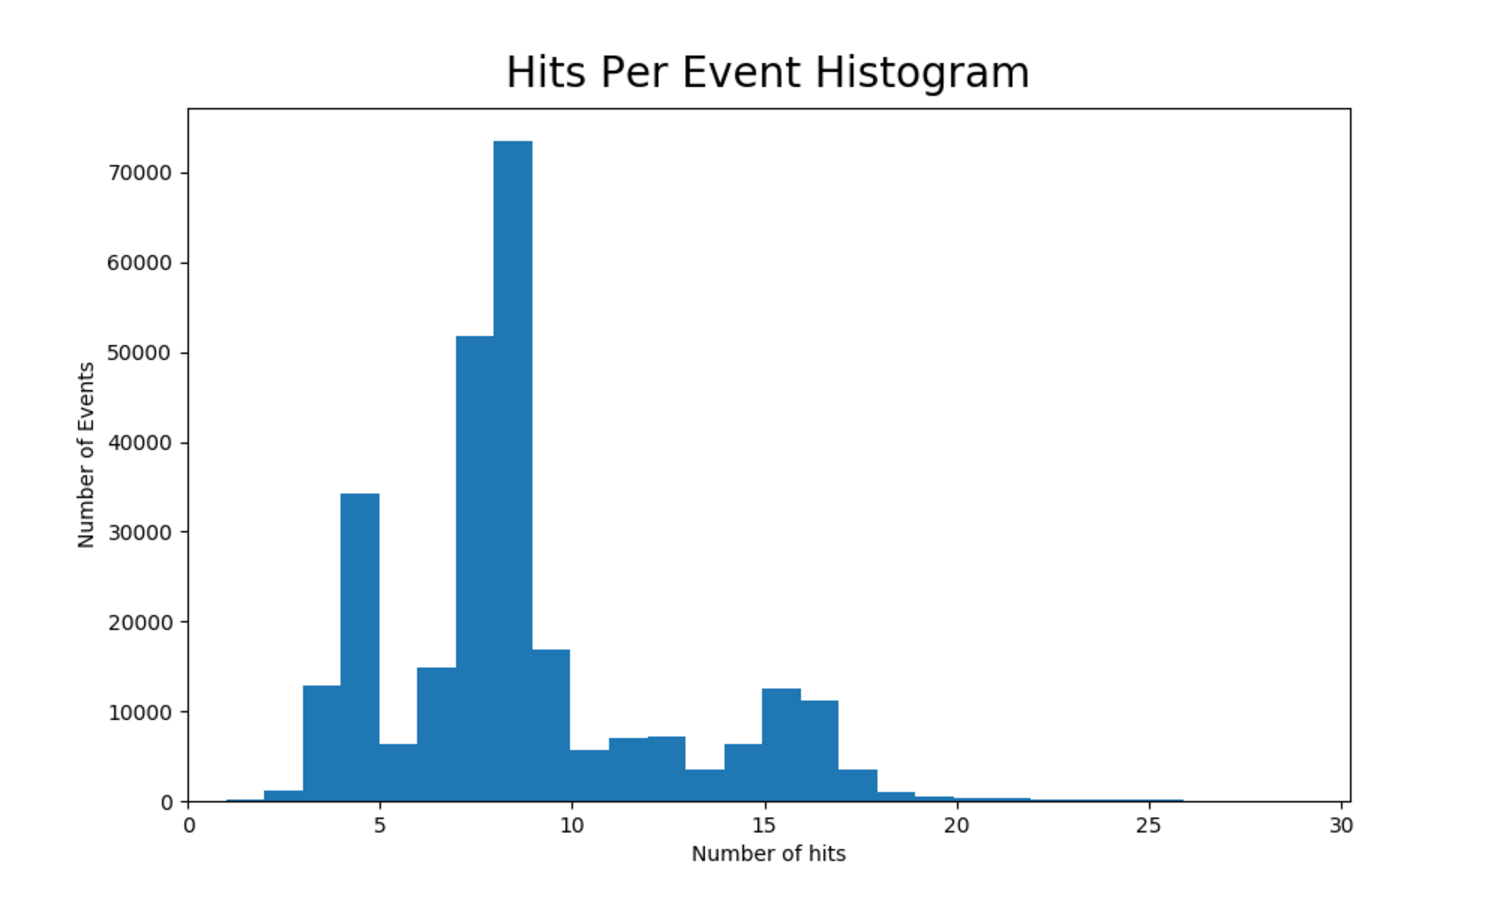
\includegraphics[scale=0.5]{pictures/Hits_per_event.pdf}
\caption{Number event with a certain amount of hits}
\label{fig:hits_per_event}
\end{figure}

This preliminary analysis can be concluded with a first estimate of the efficiency of the various chambers: requiring that a chamber "spots a signal" when it register at least 3 hits in 3 different layers, the table \ref{tab:chamber_efficiency} can be built, where the conditional probabilities of having one of the chamber of the couple "good", when the other is too, are reported. In general, as can be seen, the results are fairly good, in the sense that in most cases, if a chamber spot the muon, the other is no less. The problem arises in data regarding chamber 0, less efficient of the other ones, as justified above (because of the dead cells). \\

\begin{table}[!h]
\centering
\begin{tabular}{c|c}
\toprule
Good\_ch0 $\mid$ Good\_ch1 &  76.42\% \\
\midrule
Good\_ch1 $\mid$ Good\_ch0 &  87.64\% \\
\midrule
Good\_ch2 $\mid$ Good\_ch3 &  89.45\% \\
\midrule
Good\_ch3 $\mid$ Good\_ch2 &  86.60\% \\
\bottomrule
\end{tabular}
\begin{tabular}{c|c}
\toprule
Good\_ch0 $\mid$ Good\_ch2 &  27.41\% \\
\midrule
Good\_ch2 $\mid$ Good\_ch0 &  34.91\% \\
\midrule
Good\_ch1 $\mid$ Good\_ch3 &  30.60\% \\
\midrule
Good\_ch3 $\mid$ Good\_ch1 &  32.89\% \\
\bottomrule
\end{tabular}
\caption{Conditional probability using neighbour chamber as a tag}
\label{tab:chamber_efficiency}
\end{table}

For the pairs of chambers in the table on the right, instead, such low values of the percentages can be traced to the fact that they are considering detectors separated by about a meter away, while the pairs in the table on the left identify chamber directly in contact with each other.\\
Muons that cross the detector with directions that are too "inclined", compared to the vertical one, can in fact be spotted from the upper chambers and not from the lower ones.\\


\chapter{Tracks recostruction}

Before starting with the technical part, i.e. the explanation of how tracks are reconstructed, it is appropriate to go into detail of the geometric configuration of the system.\\
These detectors are drift chambers of square shape of dimensions 700x700 mm, arranged one above the other, as shown above in figure \ref{fig:2019_esp_setup}, and are oriented two by two, long x and y space directions. In particular, chambers 0 and 2 report the information along x axis, while chambers 1 and 3 along y axis.\\
In this second part, the algorithm works on events file, the one produced after preprocessing phase: a txt file in which every line represent an entire event (no longer a single hit) with all the coordinates of collected signal and the left-right ambiguity not resolved yet. Then, the events are read line by line, and rewritten each in a dataframe by itself in such a way to be able to work more easily on the single one (and because, in an eventual "global" dataframe, every event should have a different number of columns).\\


\section{Projection recostruction}

Because, as explained above, detectors of this type collect information on the passage of the muon only in two dimensions (x/y and z), it is not possible to reconstruct the trace with data belonging to only one chamber, and this is why these detectors are arranged in different directions. A "good event", in this case, consists of an alignment in each of the four chambers, so that we can fit the projections on xz/yz plan before, and then exploit the results to get three dimensional track.\\ 
So, the algorithm, as said, works event by event, doing a preliminar selection (to check its goodness, and then, for every chamber,  performing a local linear fit to determinate the three or four points that are the "best aligned" (resolving left-right ambiguity too), and distinguishing signal points from background (phantom) points.\\
Because both projection (xz and yz) of the track are needed to get three dimensional reconstruction, it is requested that all four chambers are good, and this request is placed in the following manner:
\begin{itemize}
\item[-] Chambers with too few points, or with too much noise, are excluded. To be more specific, the request is that the number of signal is included between 3 and 7 (with too confusing events it is hard to spot the best local alignment).
\item[-] Chambers with more than 3 couple of hits in the same layer of cell are excluded.
\item[-] We ask for different signals in at least three different layers, to have enough points for the linear interpolation.
\end{itemize}
The request to have a good event is, indeed, quite restrictive (because it tends to exclude many events) despite it limits to ask for the bare minimum for a local fit in each chamber: this could be mainly due to the selection of the previous phase and to the fact that just for one bad chamber the event is lost. Despite all, anyway, thank to the large amount of data collected, the analysis will be done with a good number of tracks (very clean), more than enough for a consistent statistic.\\
The next step is to study, chamber by chamber, the points distribution, so as to identify the best alignment. This research is done considering all the possible combination of three or four points (with left-right ambiguity unresolved) and performing for each one a linear fit, and, in the end, considering only the best one, discriminating them based on the chi square. In particular it is appropriate to specify that the algorithm uses weighted interpolation, in such a way to take into consideration a minimum error on the position of the points in the chamber, a small contribution that could be due to an incorrect estimate of the drift time (in the computing of time pedestal or in the measure itself).\\
Once determined, for each detector, we proceed by reconstructing the global projections of the muon track: the chambers are considered two by two depending on the plan on which they collects information. At this point, all that remains is to perform a new linear interpolation 
of which an example is shown in figure \ref{fig:glob_proj_ex}.\\

\begin{figure}[hbtp]
\centering
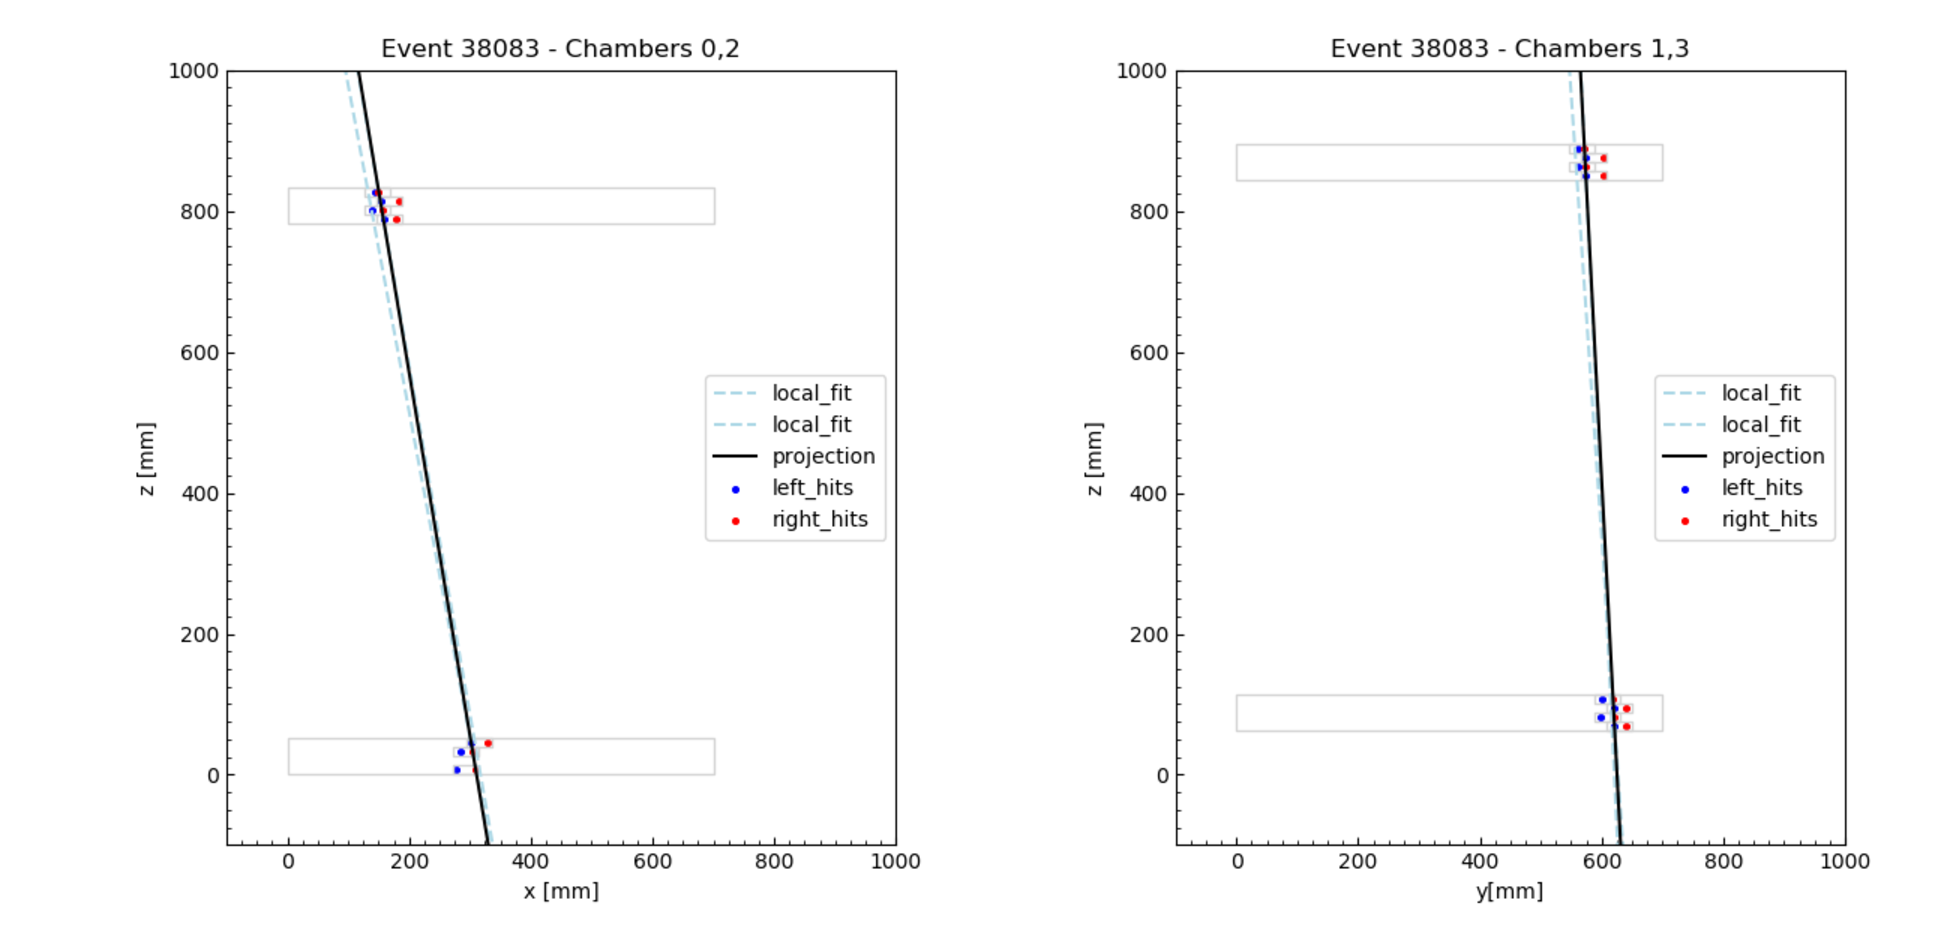
\includegraphics[scale=0.4]{pictures/example_track2D.pdf}
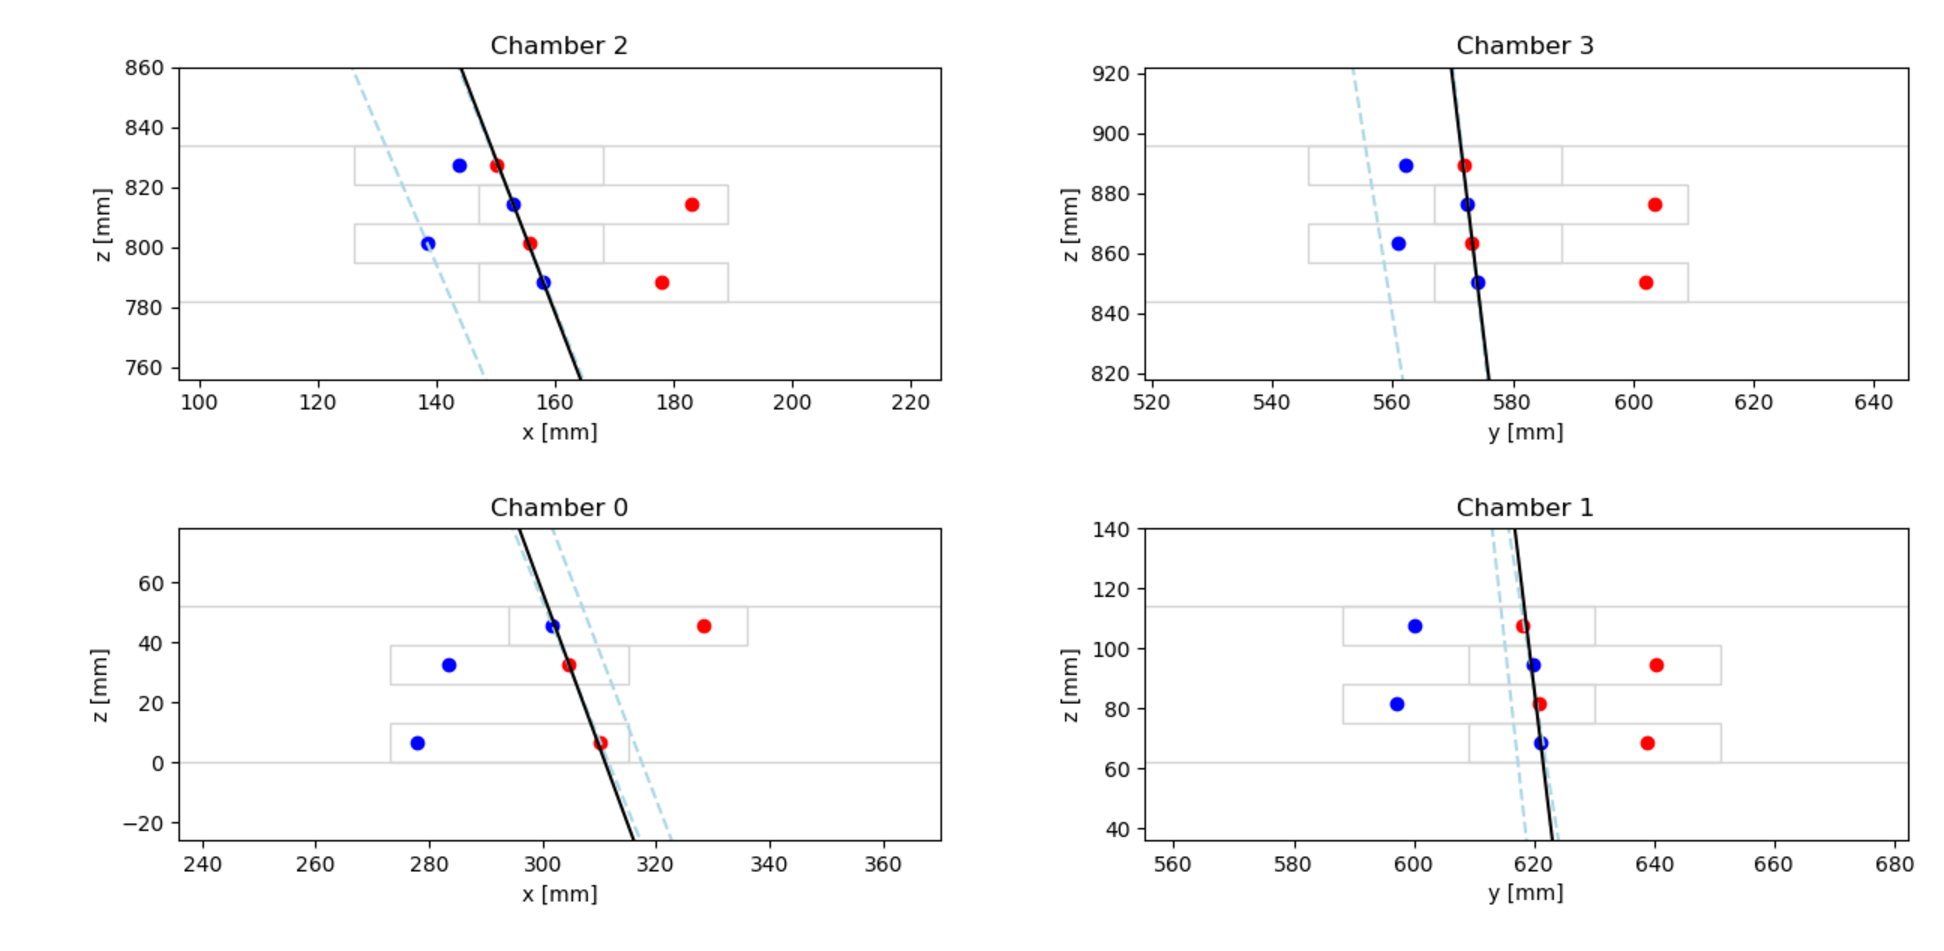
\includegraphics[scale=0.4]{pictures/example_track2D_dets.pdf}
\caption{Global and local projections of muon track}
\label{fig:glob_proj_ex}
\end{figure}


\section{Calibration}

As all the experimental systems, this one needs a calibration phase too.\\
Unlike when it was used as a test beam, it is not longer possible to collect data set specifically for this operations because, with the chambers facing upwards, it would be necessary to install a muon source on the roof of the laboratory, which continuously sends signals to the detectors. Therefore the same data collected for the analysis will undergo a preliminary control phase, necessary for an estimate of the calibration parameters of the system.\\
There are two main effects that contribute to possible systematic errors on points' positions: an incorrect estimate of the electrons drift velocity and an overestimation/underestimation of the time pedestal. Actually, known value of drift speed is:
\[ v_{drift} = XCELL/(2*T_{max}) = 42mm/(2*390ns) = 0.05385\hspace{1mm} mm/ns \]
while time pedestal are calculated with the method discussed above, and their distribution is represented in figure \ref{fig:DRIFT_TIMES}.\\
To estimate calibration parameters, than, we can proceed analyzing residuals of the points used to interpolate the track, defined as the difference between the module of the distance hit-wire and the module of the distance fit-wire (estrapolated from the global fit line). In particular, if the time pedestal is underestimated/overestimated, this residuals on average will be higher or smaller than zero: this can be checked computing 1D histogram of residuals for every chamber (as they may need different corrections). Results, reported in figure \ref{fig:res1D} and in table \ref{tab:res1D} (where gaussian interpolation parameters of histograms are collected), denote that, for this data set, no corrections are needed, because distributions' centroid are compatible with zero.\\

\begin{figure}[hbtp]
\begin{minipage}[c]{0.6\textwidth}
\centering
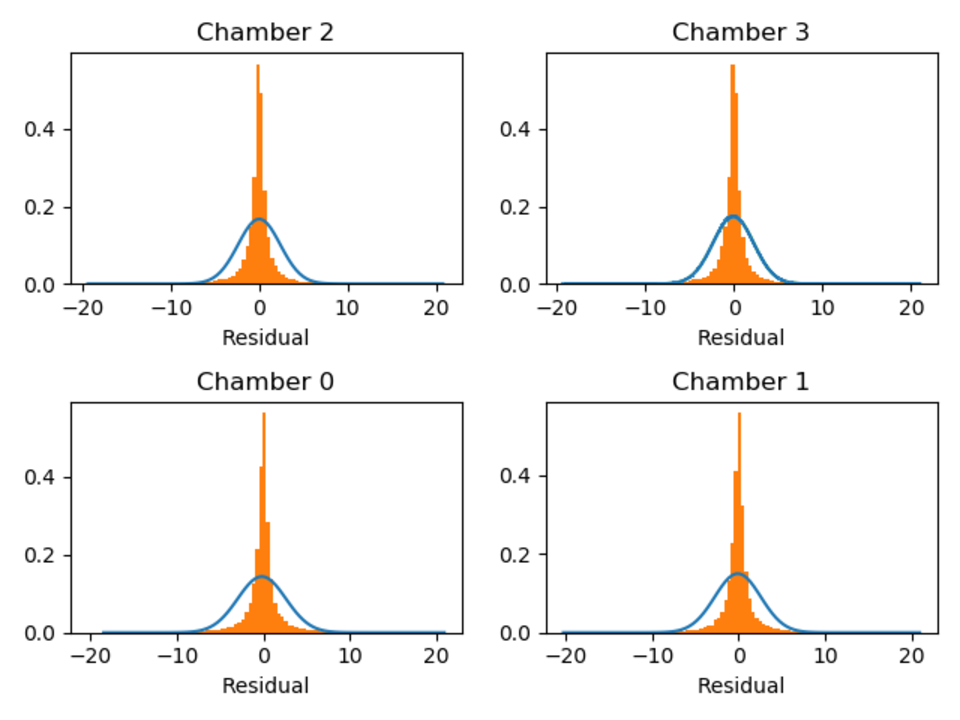
\includegraphics[scale=0.6]{pictures/Residuals_1D.pdf}
\caption{Residuals 1D of the four chambers}
\label{fig:res1D}
\end{minipage}\quad
\begin{minipage}[c]{0.4\textwidth}
\begin{tabular}{c | c  c}
\toprule
 \textbf{Chamber} & $\bm{\mu}$\textbf{ [mm]} & $\bm{\sigma}$\textbf{ [mm]}\\
0 & -0.17 & 2.8\\
1 & -0.11 & 2.7\\
2 & -0.02 & 2.38\\
3 &-0.09  & 2.29\\
\bottomrule
\end{tabular}
\caption{Parameters of the 1D residuals histograms}
\label{tab:res1D}
\end{minipage}
\end{figure}

If it were the drift speed to be wrong, the further away you are from the wire, the more the residuals will be on average different from zero. This analysis can be computed checking for a trend in the two-dimensional distribution of the residuals, reported in figure \ref{fig:res2D}, in which highlighted points represent the average and the standard deviation of data in a small region of the graphic (useful for a better estimate of the general trend).\\
To be more precise, in the graph \ref{fig:res2D}, are represented residuals (defined as $|x_{hit}-x_{wire}|-|x_{fit}-x_{wire}|$ in function of the distance of the hit from the wire.\\

\begin{figure}[hbtp]
\centering
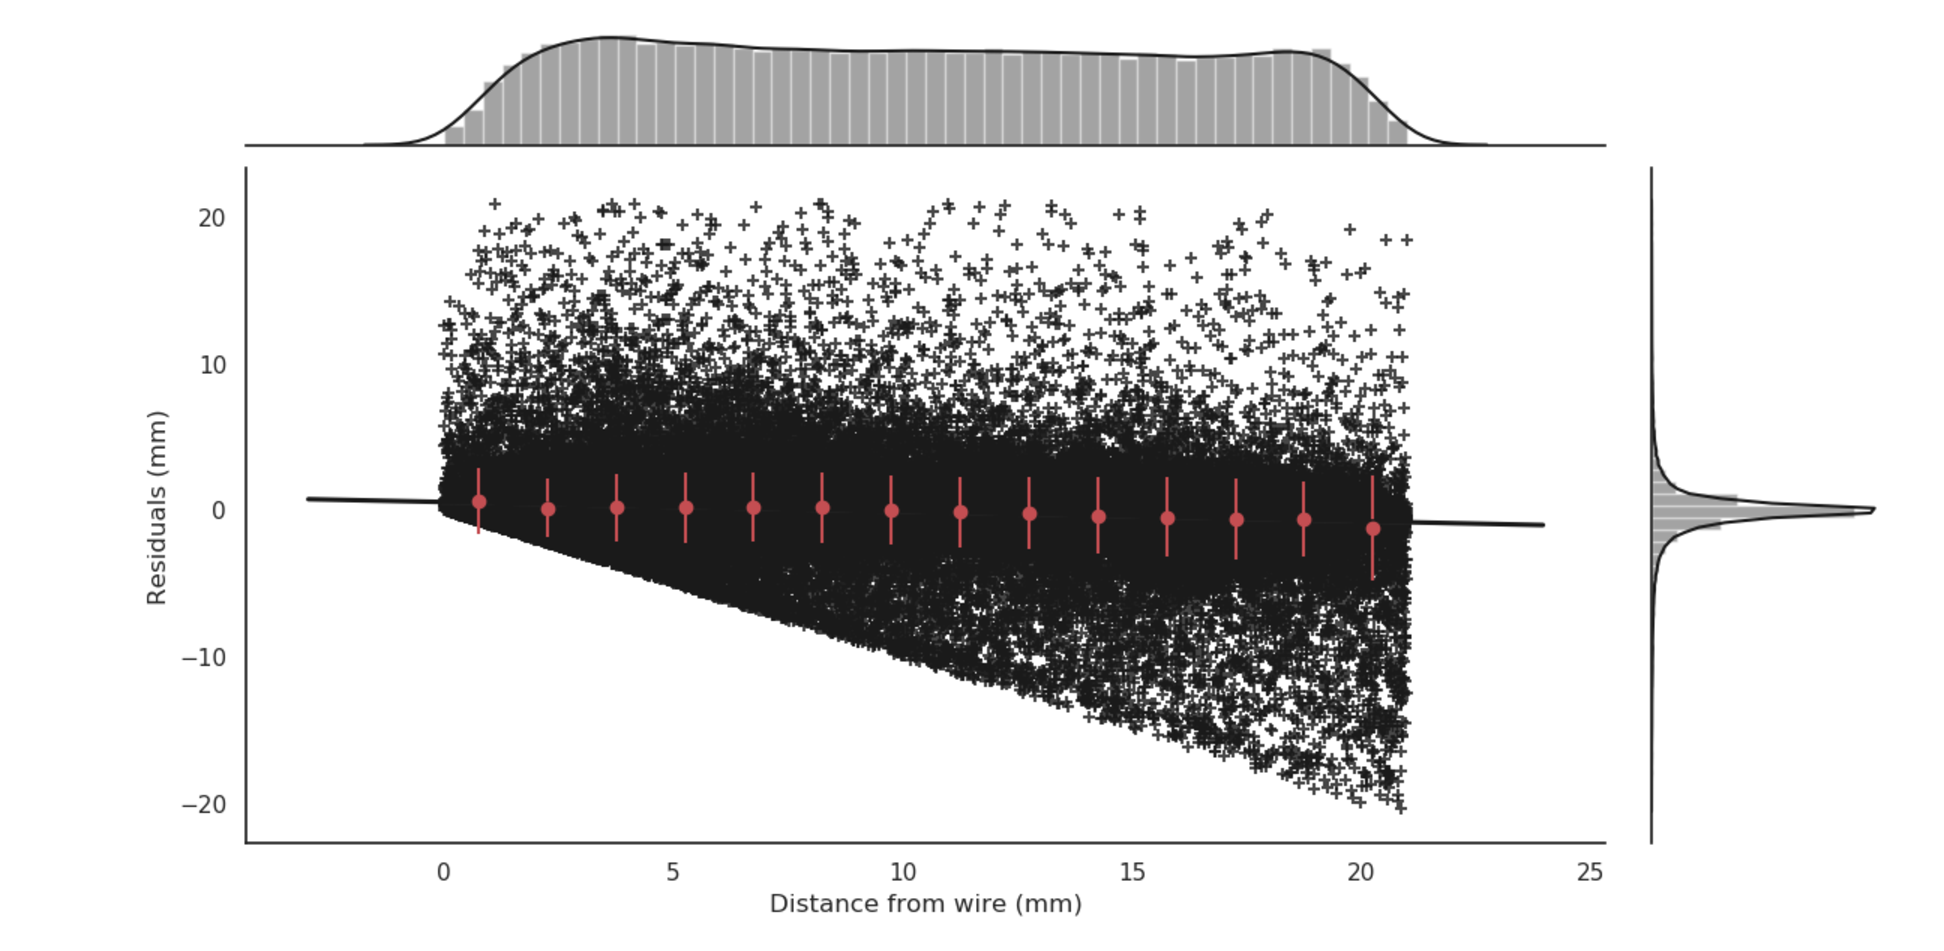
\includegraphics[scale=0.4]{pictures/Residuals_2D.pdf}
\caption{Residuals 2D}
\label{fig:res2D}
\end{figure}

\begin{table}[!h]
\centering
\begin{tabular}{c  c}
\toprule
 \textbf{Slope} & \textbf{Intercept [mm]}\\
-0.066 & -0.584 \\
\bottomrule
\end{tabular}
\caption{Parameters of the linear interpolation}
\label{tab:res2D_analysis}
\end{table}

Table \ref{tab:res2D_analysis} collects linear fit parameters of the line present in the graph. From these parameters, we see how the researched trend in the distribution is not actually present (slope is compatible with zero) and therefore, from this point of view too, no coordinates correction is necessary.\\


\section{3D recostruction}

Once the projection of the tracks have been calculated (and eventually corrected the positions of the points if the calibration revealed some incongruity), purely geometric relationships are exploited to reconstruct the passage of the muon in three dimensions. In particular, we consider the plans generated by the two projection and the direction of the wires they refers to (xz plan and y axis or yz plan and x axis), and take the intersection.\\
The result of the method (for the event studied in the previous chapter) is the following:

\begin{figure}[hbtp]
\centering
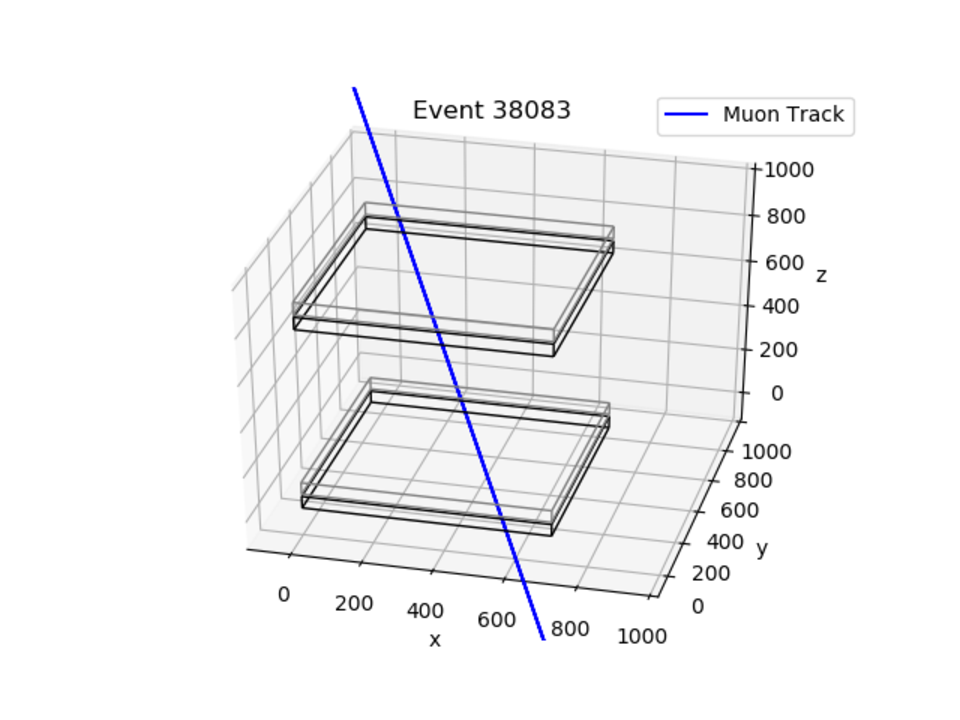
\includegraphics[scale=0.5]{pictures/Track_3D.pdf}
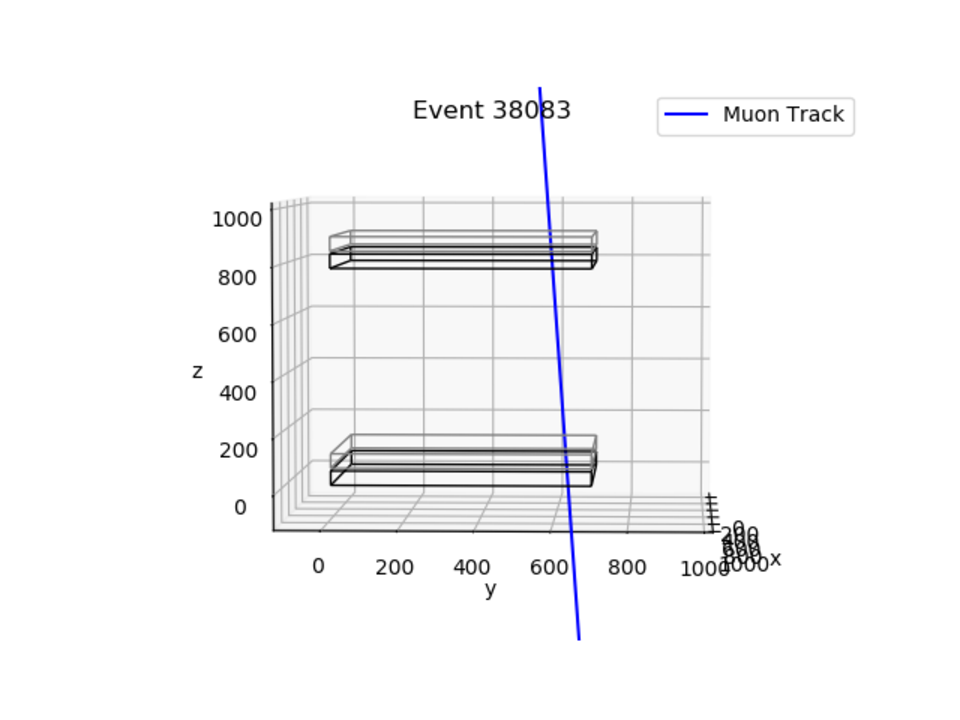
\includegraphics[scale=0.5]{pictures/Track_3D_2.pdf}
\caption{3D recostruction of muon track}
\label{fig:3D_track}
\end{figure}




\chapter{Analysis}

In this chapter, some other possible analysis will be shown, after full track recostruction. In particular we will linger on the angular resolution of the system and on the frequency with which good events are recognized.\\

\section{Angular resolution}

A useful study to do to test system's limits is to check its angular resolution. Basically, knowing slope values of global fit lines, it is possible to trace the maximum track's inclinations with which the chambers can work, and rebuild the entire muon route. Defined the angle that will be represented in the figure as the one between the line and the z axis (i.e. the vertical direction), in both sides xy and xz, the following results were obtained , in plot \ref{fig:angles} e in table \ref{tab:angles}. \\
\begin{figure}[hbtp]
\begin{minipage}[c]{0.6\textwidth}
\centering
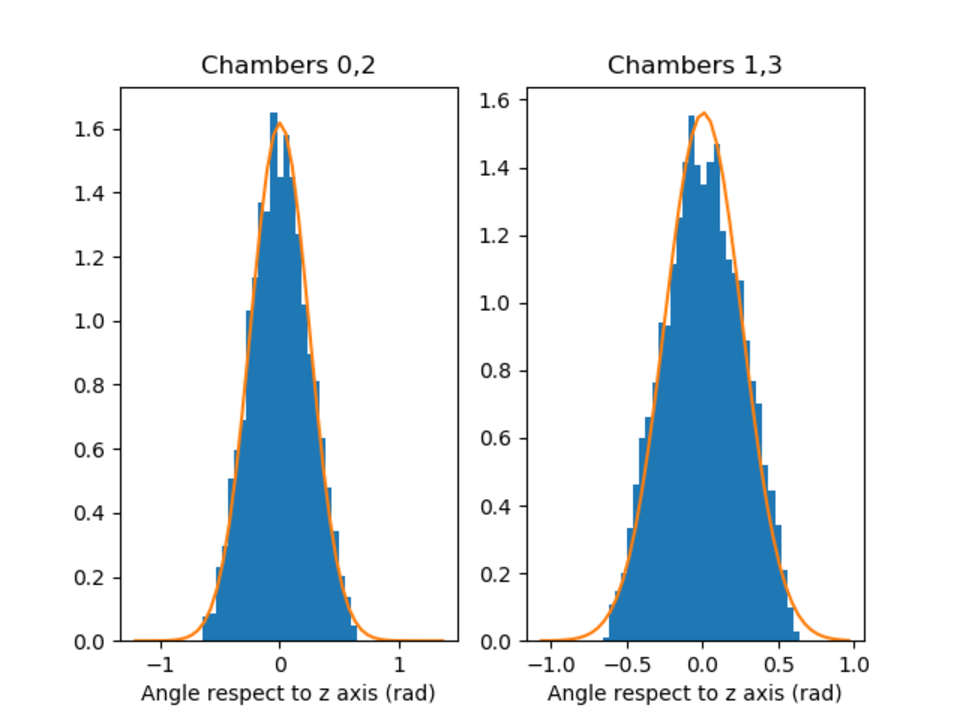
\includegraphics[scale=0.6]{pictures/Angles.pdf}
\caption{Graphical representation of angular resolution of the detectors}
\label{fig:angles}
\end{minipage} \quad
\begin{minipage}[c]{0.4\textwidth}
\begin{tabular}{c | c  c}
\toprule
 \textbf{Side} & $\bm{\mu}$\textbf{[rad]} & $\bm{\sigma}$\textbf{[rad]}\\
xz & 0.0037 & 0.25\\
yz & 0.0044 & 0.26\\
\bottomrule
\end{tabular}
\caption{Parameters of the interpolation}
\label{tab:angles}
\end{minipage}
\end{figure}

A good estimate of the angular resolution can be obtained thank to the calculation of the FWHM (= $2\sqrt{2\ln 2}\cdot\sigma$, full width at half maximum) of the gaussian interpolations of the histograms. Final results are reported in table \ref{tab:angular_resolution}.
\begin{table}[hbtp]
\centering
\begin{tabular}{c c c}
\toprule
\textbf{Side} & \textbf{FWHM (rad)} & \textbf{Resolution (degrees)}\\
\midrule
xz & 0.59 & 33.80\\
yz & 0.61 & 34.95\\
\bottomrule
\end{tabular}
\caption{Angular resolution}
\label{tab:angular_resolution}
\end{table}

As it can be read, the system has a fairly wide angular resolution, about 35° for side. It is important to remember that muons that pass trough the chambers at an excessive angle, mark diagonal patterns of cells, unusable for the application of the Talete's theorem for the meantimer algorithm.\\


\section{Some statistics}

Below (table \ref{tab:stats}), are reported some useful information, like the number of the events recostructed in the first part of the paper, referred to those that the second part judged "good".\\

\begin{table}[htbp] 
\centering
\begin{tabular}{c|c}
\toprule
\textit{Total events analyzed} & 66541\\
\midrule
\textit{Good events selected} & 8080 (12.14 \%)\\
\bottomrule
\end{tabular}
\caption{Selection efficiency of the events}
\label{tab:stats}
\end{table}

Good event's percentage is actually rather a bit small, but, as said before, algorithm requests in the second part are very restrictive, in the sense that events are easily ruled out: if just one of the chambers contains too much noise compared to the others the event will be rejected. But, as binding it is, the request to have all four detectors "good" is strictly necessary to reconstruct the trace three-dimensionally. And then almost all the accepted events are like the one shown in figure \ref{fig:glob_proj_ex}, in the sense that they are clean and defined signs in which the different interpolations are nearly perfectly overlapped.\\
However the information loss caused by dead cells in chamber 0 must not be forgotten because, in such a delicate method, can be decisive in establishing the goodness of the detector. \\
To quantify how many "almost good" events the algorithm processed, i.e. the events rejected because of an error in just one of the chambers, it is sufficient to check table \ref{tab:rejected_chamber}.\\

\begin{table}[htbp]
\centering
\begin{tabular}{c|c}
\toprule
\textit{Events rejected (only) by bad chamber 0} & 2322 (3.49\%) \\
\midrule
\textit{Events rejected (only) by bad chamber 1} & 717 (1.08\%) \\
\midrule
\textit{Events rejected (only) by bad chamber 2} & 281 (0.42\%) \\
\midrule
\textit{Events rejected (only) by bad chamber 3} & 1187 (1.78\%) \\
\bottomrule
\end{tabular}
\caption{Events rejected by one "bad" chamber}
\label{tab:rejected_chamber}
\end{table}

As to be expected, is precisely the chamber 0 that is responsible of the rejection of many events.\\
However, to gain greater "bidimensional" statistics, intended as restricted to xz and yz projection (for example in the computation of the angular resolution or in the calibration phase), it is sufficient a slight modification of the code, a small change on the condition of acceptance, asking that just a couple of chambers (and not both) can be fitted for a global track.\\




\chapter{Conclusions}
The objective of this project was to develop a reconstruction algorithm flexible and fast enough to study data of cosmic muons taken at Legnaro's laboratories. \\
To summarize what has been done: raw data in hexadecimal format were converted and grouped by collection time and the geometry of the system has been exploited to compute the time pedestal of the events to explicit the exact position of the passage of the particle; then, the events created in such way have been analyzed to check their goodness and to find the best local alignment pattern for the points in every chamber; finally the points found in the previous phase have been linearly interpolated to compute the global projections of the real muon trace, which will be reconstructed thank to them.\\
During this work, the algorithm was tested on data collected on both the experimental setups described in chapter \ref{ch:exp_setup} (test beam setup and cosmic setup) with satisfying results in terms of computational resources and track reconstructed. As explained above, the requests imposed on the events to be good may appear too restrictive, but they are necessary to isolate clear tracks like the one shown in \ref{fig:glob_proj_ex} and \ref{fig:3D_track}.\\
Anyhow, except for the problems with chamber 0, we can conclude that the algorithm was able to extrapolate a good number of events from the collected data, allowing a complete statistical analysis (and calibration of the system) on them.\\




\addcontentsline{toc}{chapter}{References}
\clearpage

\begin{thebibliography}{1}
\bibitem{bib:lessons_in_coding} Henley A. J., Wolf D. (2018), \textit{Learn Data Analysis with Python: Lessons in Coding}, Apress 
\bibitem{bib:python_data_analysis} McKinney W. (2012), \textit{Python for Data Analysis}, O'Reilly 
\bibitem{bib:det_grupen} Grupen C., Shwartz B. (2008), \textit{Particle Detectors}, 2nd edition, Cambridge 
\bibitem{bib:det_drift} Blum W., Riegler W., Rolandi L. (2008), \textit{Particle Detection with Drift Chambers}, Springer
\bibitem{bib:CMS} CMS Collaboration (2014), \textit{The performance of the CMS muon detector in proton–proton collisions at $\sqrt{s}$ = 7 TeV at the LHC}, CMS-MUO-11-001, Journal of Instrumentation
\bibitem{bib:cosmic_muons} Liu L. (2007), \textit{The Speed and Lifetime of Cosmic Ray Muons}, MIT Undergraduate
\bibitem{bib:low_emittance_muon_collider} Boscolo M. et al. (2018), \textit{Muon Accumulator Ring Requirements for a Low Emittance Muon Collider from Positron in Target}, Vancouver, IPAC2018
\bibitem{bib:gas_det} Krammer M., \textit{Gaseous Detectors}, Institute for High Energy Physics, Vienna, Austria
\bibitem{bib:LEMMA} Boscolo M. (2018), \textit{LEMMA}, Padova, ARIES Muon Collider Workshop
\end{thebibliography}





\end{document}






